%!TEX root = main.tex
\begin{theorem}[Representation]\label{th:representaiton}
\todo[inline]{Representation theorem: can uniquely define kernel $P^{\RV{X}|\RV{Y}}$ with $P^{\RV{Z}|\RV{Y}}$ and $P^{\RV{X}|\RV{Z}\RV{Y}}$ }
\end{theorem}


\subsection{Probability Theory}

Given a set $A$, a $\sigma$-algebra $\mathcal{A}$ is a collection of subsets of $A$ where
\begin{itemize}
	\item $A\in \mathcal{A}$ and $\emptyset\in \mathcal{A}$
	\item $B\in \mathcal{A}\implies B^C\in\mathcal{A}$
	\item $\mathcal{A}$ is closed under countable unions: For any countable collection $\{B_i|i\in Z\subset \mathbb{N}\}$ of elements of $\mathcal{A}$, $\cup_{i\in Z}B_i\in \mathcal{A}$ 
\end{itemize}

A measurable space $(A,\mathcal{A})$ is a set $A$ along with a $\sigma$-algebra $\mathcal{A}$. Sometimes the sigma algebra will be left implicit, in which case $A$ will just be introduced as a measurable space.

\paragraph{Common $\sigma$ algebras}

For any $A$, $\{\emptyset,A\}$ is a $\sigma$-algebra. In particular, it is the only sigma algebra for any one element set $\{*\}$.

For countable $A$, the power set $\mathscr{P}(A)$ is known as the discrete $\sigma$-algebra.

Given $A$ and a collection of subsets of $B\subset\mathscr{P}(A)$, $\sigma(B)$ is the smallest $\sigma$-algebra containing all the elements of $B$. 

Let $T$ be all the open subsets of $\mathbb{R}$. Then $\mathcal{B}(\mathbb{R}):=\sigma(T)$ is the \emph{Borel $\sigma$-algebra} on the reals. This definition extends to an arbitrary topological space $A$ with topology $T$.

A \emph{standard measurable set} is a measurable set $A$ that is isomorphic either to a discrete measurable space $A$ or $(\mathbb{R}, \mathcal{B}(\mathbb{R}))$. For any $A$ that is a complete separable metric space, $(A,\mathcal{B}(A))$ is standard measurable. 

Given a measurable space $(E,\mathcal{E})$, a map $\mu:\mathcal{E}\to [0,1]$ is a \emph{probability measure} if
\begin{itemize}
	\item $\mu(E)=1$, $\mu(\emptyset)=0$
	\item Given countable collection $\{A_i\}\subset\mathscr{E}$, $\mu(\cup_{i} A_i) = \sum_i \mu(A_i)$
\end{itemize}

Write by $\Delta(\mathcal{E})$ the set of all probability measures on $\mathcal{E}$.

A particular probability measure we will often discuss is the \emph{Dirac measure}. For any $x\in X$, the Dirac measure $\delta_x\in \Delta(\sigalg{X})$ is the probability measure where $\delta_x(A)=0$ if $x\not\in A$ and $\delta_x(A)=1$ if $x\in A$.

Given another measurable space $(F,\mathcal{F})$, a \emph{stochastic map} or \emph{Markov kernel} is a map $\kernel{M}:E\times\mathcal{F}\to [0,1]$ such that
\begin{itemize}
	\item The map $\kernel{M}(\cdot;A):x\mapsto \kernel{M}(x;A)$ is $\mathcal{E}$-measurable for all $A\in \mathcal{F}$
	\item The map $\kernel{M}_x:A\mapsto \kernel{M}(x;A)$ is a probability measure on $F$ for all $x\in E$
\end{itemize}

Extending the subscript notation, for $\kernel{C}:X\times Y\to \Delta(\mathcal{Z})$  and $x\in X$ we will write $\kernel{C}_{x,\cdot}$ for the ``curried'' map $y\mapsto \kernel{C}_{x,y}$. If $\kernel{C}$ is a Markov kernel with respect to $(X\times Y, \sigalg{X}\otimes\sigalg{Y}),(Z,\sigalg{Z})$ then it is straightforward to show that $\kernel{C}_{x,\cdot}$ is a Markov kernel with respect to $(Y,\sigalg{Y}),(Z,\sigalg{Z})$.

This yields the notational conventions for arbitrary kernel $\kernel{C}$:

\begin{itemize}
	\item $\kernel{C}$ with no subscripts is a Markov kernel
	\item $\kernel{C}_{\cdot,a,b}$ with at least one $\cdot$ subscript is a Markov kernel
	\item $\kernel{C}_y$ with no $\cdot$ subscripts is a probability measure
\end{itemize}

The map $x\mapsto \kernel{M}_x$ is of type $E\to \Delta(\mathcal{F})$. We will abuse notation somewhat to write $\kernel{M}:E\to \Delta(\mathcal{F})$. In this sense, we view Markov kernels as maps from elements of $E$ to probability measures on $\mathcal{F}$. This is simply a convention that helps us to think about constructions involving Markov kernels, and it is equally valid to view Markov kernels as maps from elements of $\mathcal{F}$ to measurable functions $E\to[0,1]$, a view found in \citet{clerc_pointless_2017}, or simply in terms of their definition above.

Given an indiscrete measurable space $(\{*\},\{\{*\},\emptyset\})$, we identify Markov kernels $\kernel{N}:\{*\}\to \Delta(\mathcal{E})$ with the probability measure $\kernel{N}_*$. In addition, there is a unique Markov kernel $\stopper{0.2}:E\to \Delta(\{\{*\},\emptyset\})$ given by $x\mapsto \delta_*$ for all $x\in E$ which we will call the ``discard'' map.

Two Markov kernels $\kernel{M}X\to \Delta(\sigalg{Y})$ and $\kernel{N}:X\to \Delta(\sigalg{Y})$ are equal iff for all $x\in X$, $A\in \sigalg{Y}$
\begin{align}
	\kernel{M}_x(A) = \kernel{N}_x(A)
\end{align}

We will typically be more concerned with ``almost sure'' equality than exact equality, which will be defined later.

\subsection{Product Notation}\label{ssec:product_notation}

Probability measures, Markov kernels and measurable functions can be combined to yield new probability measures, Markov kernels or measurable functions. Given $\mu\in \Delta(\mathcal{X})$, $\RV{T}:Y\to T$, $\kernel{M}:X\to \Delta(\sigalg{Y})$ and $\kernel{N}:Y\to \Delta(\sigalg{Z})$ define:

The \textbf{measure-kernel} product $\mu \kernel{M}:\sigalg{Y}\to [0,1]$ where for all $A\in\sigalg{Y}$,

\begin{align}
\mu\kernel{M} (A) := \int_X \kernel{M}_x (A) d\mu(x)
\end{align}

The \textbf{kernel-function} product $\kernel{M} \RV{T}:X\to T$ where for all $x\in X$:

\begin{align}
\kernel{M}\RV{T}(x) := \int_Y T(y) d\kernel{M}_x(y)
\end{align}


The \textbf{kernel-kernel} product $\kernel{M}\kernel{N}:X\to \Delta(\sigalg{Z})$ where for all $x\in X$, $A\in \sigalg{Z}$:

\begin{align}
(\kernel{M}\kernel{N})_x(A) &:= \int_Y \kernel{N}_y(A) d\kernel{M}_x(y)
 \end{align} 

All kernel products are associative \citep{cinlar_probability_2011}. An intuition for this notation can be gained from thinking of probability measures $\mu\in \Delta(\mathcal{X})$ as row vectors, Markov kernels $\kernel{M},\kernel{N}$ as matrices and measurable functions $\RV{T}:Y\to T$ as column vectors and kernel products are vector-matrix and matrix-matrix products. If the $X,Y,Z$ and $T$ are discrete spaces then this analogy is precise.

Finally, the \textbf{tensor product} $\kernel{M}\otimes \kernel{N}:X\times Y\to \Delta(\sigalg{Y}\otimes\sigalg{Z})$ is yields the kernel that applies $\kernel{M}$ and $\kernel{N}$ ``in parallel''. For all $x\in X$, $y\in Y$, $G\in \sigalg{Y}$ and $H\in \sigalg{Z}$:

\begin{align}
(\kernel{M}\otimes \kernel{N})_{x,y}(G\times H) := \kernel{M}_x(G)\kernel{N}_y(H)
\end{align}

\subsection{String Diagrams}\label{ssec:mken_diagrams}

Some constructions are unwieldly in product notation; for example, given $\mu\in \Delta(\mathcal{E})$ and $\kernel{M}:E\to (\mathcal{F})$, it is not straightforward to write an expression using kernel products and tensor products that represents the ``joint distribution'' given by $A\times B\mapsto \int_A \kernel{M}(x;B)d\mu$.

An alternative notation known as \emph{string diagrams} provides greater expressive capability than product notation while being more visually clear than integral notation. \citet{cho_disintegration_2019} provides an extensive introduction to string diagram notation for probability theory.

Key features of string diagrams include:
\begin{itemize}
	\item String diagrams as they are used in this work can always be interpreted as a mixture of kernel-kernel products and tensor products of Markov kernels
	\item String diagrams are the subject of a coherence theorem: two string diagrams that differ only by planar deformation are always equal \citep{selinger_survey_2010}. This also holds for a number of additional transformations detailed below
	\begin{itemize}
		\item Informally, diagrams that look like they should be the same are in fact the same
	\end{itemize}
\end{itemize}

\subsubsection{Elements of string diagrams}

The basic elements of a string diagram are Markov kernels. Diagrams representing Markov kernels can be assembled into larger diagrams by taking regular products or tensor products.

Indiscrete spaces play a key role in string diagrams. An indiscrete space is any one element measurable space $(\{*\},\{\emptyset,\{*\}\})$ which admits the unique probability measure $\mu:\{\emptyset,\{*\}\}\to(0,1)$ given by $\mu(\emptyset)=0$, $\mu(\{*\})=1$. Any probability measure $\mu\in \Delta(\sigalg{X})$ can be interpreted as a Markov kernel $\mu':\{*\}\to \Delta(\mathcal{X})$ where $\mu'_*=\mu$ (note that $*$ is the \emph{only} argument $\mu'$ can be given).


A Markov kernel $\kernel{M}:X\to \Delta(\mathcal{Y})$ can always be represented as a rectangular box with input and output wires labeled with the relevant spaces:

\begin{align}
\begin{tikzpicture}
\path (0,0) node (A) {$X$}
++(0.75,0) node[kernel] (B) {$\kernel{M}$}
++(0.75,0) node (C) {$Y$};
\draw (A) -- (B) -- (C);
\end{tikzpicture}
\end{align}

Note that we will later substitute labelling wires with spaces for labelling them with random variable names.

Probability measures are kernels with an indiscrete domain $\mu \in \Delta(\mathcal{X})$ can be written as triangles:
\begin{align}
\begin{tikzpicture}
\path (0,0) node[dist] (B) {$\mu$}
++(0.75,0) node (C) {$X$};
\draw (B) -- (C);
\end{tikzpicture}\label{eq:prob_meas_sd}
\end{align}

Note that Eq \ref{eq:prob_meas_sd} technically represents a Markov kernel $\mu':\{*\}\to\Delta(\mathcal{X})$, but for our purposes this distinction isn't practically important.

We do \emph{not} define kernel-function products for string diagrams. While kernel-kernel products always yield Markov kernels as a result, and measure-kernel products can be reinterpreted as kernel-kernel products, kernel-function products do not admit such a reinterpretation. \citet{cho_disintegration_2019} defines the operation of \emph{conditioning} using kernel-function products, but this will take extra work to incorporate into our notation which hasn't yet been done.

\paragraph{Elementary operations}

Kernel-kernel products have a visually similar representations in string diagram notation to the previously introduced product notation. Given $\kernel{M}:X\to\Delta(\mathcal{Y})$ and $\kernel{N}:Y\to \Delta(\mathcal{Z})$, we have 

\begin{align}
\kernel{M}\kernel{N} := \begin{tikzpicture}
 \path (0,0) node (E) {$X$}
 ++ (1,0) node[kernel] (M) {$\kernel{M}$}
 ++ (1,0) node[kernel] (N) {$\kernel{N}$}
 ++(1,0) node (G) {$Z$};
 \draw (E) -- (M) -- (N) -- (G);
\end{tikzpicture}\label{eq:sd_composition}
\end{align}

For $\mu\in \Delta(\mathcal{E})$,

\begin{align}
\mu\kernel{M} &:= \begin{tikzpicture}
 \path (0,0) node[dist] (M) {$\mu$}
 ++ (1,0) node[kernel] (N) {$\kernel{M}$}
 ++(1,0) node (G) {$Z$};
 \draw (M) -- (N) -- (G);
\end{tikzpicture}
\end{align}

Tensor products in string diagram notation are represented by vertical juxtaposition. For $\kernel{O}:Z\to \Delta(\mathcal{W})$:

\begin{align}
\kernel{M}\otimes\kernel{O}&:= \begin{tikzpicture}
\path (0,0) node (E) {$X$}
++(1,0) node[kernel] (M) {$\kernel{M}$}
++(1,0) node (F) {$Y$}
(0,-0.5) node (F1) {$Z$}
++(1,0) node[kernel] (N) {$\kernel{O}$}
+(1,0) node (G) {$W$};
\draw (E) -- (M) -- (F);
\draw (F1) -- (N) -- (G);
\end{tikzpicture}
\end{align}

A space $X$ is identified with the identity kernel $\mathrm{Id}^X:X\to \Delta(\sigalg{X})$, $x\mapsto \delta_x$. A bare wire represents an identity kernel or, equivalently, the space given by its labels:

\begin{align}
\mathrm{Id}^X:=\begin{tikzpicture}
\path (0,0) node (X) {$X$}
++(2,0) node (Y) {$X$};
\draw (X) -- (Y);
\end{tikzpicture}
\end{align}

Product spaces $X\times Y$ are identified with tensor products of identity kernels $X\times Y \cong \kernel{I}^X\otimes \kernel{I}^Y$. These can be represented either by two parallel wires or by a single wire equipped with appropriate labels:
\begin{align}
X\times Y \cong \mathrm{Id}^X\otimes \mathrm{Id}^Y &:= 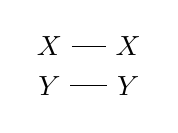
\begin{tikzpicture}
\path (0,0) node (E) {$X$}
++(1,0) node (F) {$X$}
(0,-0.5) node (F1) {$Y$}
+(1,0) node (G) {$Y$};
\draw (E) -- (F);
\draw (F1) -- (G);
\end{tikzpicture}\\
&= 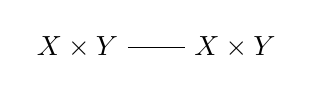
\begin{tikzpicture}
\path (0,0) node (X) {$X\times Y$}
++(2,0) node (Y) {$X\times Y$};
\draw (X) -- (Y);
\end{tikzpicture}
\end{align}

A kernel $\kernel{L}:X\to \Delta(\mathcal{Y}\otimes\mathcal{Z})$ can be written using either two parallel output wires or a single output wire, appropriately labeled:

\begin{align}
&\begin{tikzpicture}
\path (0,0) node (E) {$X$}
++ (1,0) node[kernel] (L) {$\kernel{L}$}
++ (1,0.15) node (F) {$Y$}
+(0,-0.3) node (G) {$Z$};
\draw (E) -- (L);
\draw ($(L.east) + (0,0.15)$) -- (F);
\draw ($(L.east)+ (0,-0.15)$) -- (G);
\end{tikzpicture}\\
&\equiv\\
&\begin{tikzpicture}
\path (0,0) node (E) {$X$}
++ (1,0) node[kernel] (L) {$\kernel{L}$}
++ (1.5,0) node (F) {$Y\times Z$};
\draw (E) -- (L) -- (F);
\end{tikzpicture}
\end{align}

\paragraph{Markov kernels with special notation}

A number of Markov kernels are given special notation distinct from the generic ``box'' above. This notation facilitates intuitive visual representation.

As has already been noted, the identity kernel $\textbf{Id}:X\to \Delta(X)$ maps a point $x$ to the measure $\delta_x$ that places all mass on the same point:

\begin{align}
\textbf{Id} : x\mapsto \delta_x \equiv \begin{tikzpicture}\path (0,0) node (X) {$X$} + (1,0) node (X1) {$X$}; \draw (X)--(X1); \end{tikzpicture}\label{eq:identity}
\end{align}

The identity kernel is an identity under left and right products:

\begin{align}
	(\kernel{K}\textbf{Id})_w(A) &= \int_X \textbf{Id}_x(A) d\kernel{K}_w (x) \\
							 	 &= \int_X \delta_x(A) d\kernel{K}_w(x)\\
							 	 &= \int_A d\kernel{K}_w(x)\\
							 	 &= \kernel{K}_w(A)\\
	(\textbf{Id}\kernel{K})_w(A) &= \int_X \kernel{K}_x (A) d\textbf{Id}_w(x)\\
								 &= \int_X  \kernel{K}_x(A) d\delta_w(x)\\
								 &= \kernel{K}_w(A)								  
\end{align}

The copy map $\splitter{0.1}:X\to \Delta(\mathcal{X}\times \mathcal{X})$ maps a point $x$ to two identical copies of x:
\begin{align}
 \splitter{0.1}: x\mapsto \delta_{(x,x)} \equiv 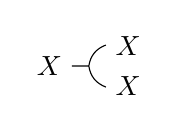
\begin{tikzpicture}
 \path (0,0) node (X) {$X$} ++ (0.5,0) coordinate (copy0) ++ (0.5,0.25) node (X1) {$X$} ++(0,-0.5) node (X2) {$X$};\draw (X)--(copy0) to [bend left] (X1) (copy0) to [bend right] (X2);
 \end{tikzpicture}\label{eq:copy}
 \end{align} 

The copy map ``copies'' its arguments to kernels or under the right product:

\begin{align}
	\int_(X\times X) \kernel{K}_{x',x''}(A) d\splitter{0.1}_x (x',x'') &= \int_(X\times X) \kernel{K}_{x',x''}(A) d\delta_{(x,x)}(x',x'')\\
															&= \kernel{K}_{x,x}(A)
\end{align}

The swap map $\sigma:X\times Y\to \Delta(\mathcal{Y}\otimes\mathcal{X})$ swaps its inputs:

\begin{align}
\sigma := (x,y)\to \delta_{(y,x)} \equiv 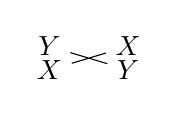
\begin{tikzpicture}
\path (0,0) node (X) {$X$}
+(1,0.3) node (X1) {$X$}
(0,0.3) node (Y) {$Y$}
+(1,-0.3) node (Y1) {$Y$};
\draw (X)--(X1) (Y) -- (Y1);
\end{tikzpicture}\label{eq:swap}
\end{align}

Under products are taken with the swap map, arguments are interchanged. For $\kernel{K}:X\times Y\to \Delta(\sigalg{Z})$ and $\kernel{L}:Z\to \Delta(\sigalg{X}\otimes\sigalg{Y})$, $A\in \sigalg{X}$, $B\in\sigalg{Y}$:

\begin{align}
	(\sigma\kernel{K})_{y,x}(A) &= \int_(X\times Y) \kernel{K}_{x',y'}(A) d\sigma_{(y,x)}(x',y') &= \int_(X\times Y) \kernel{K}_{x',y'}(A) d\delta_{(x,y)}(x',y')\\
													   &= \kernel{K}_{x,y}(A)\\
	(\kernel{L}\sigma)_{z}(B\times A) &= \int_{X\times Y} \sigma_{x',y'}(B\times A) d\kernel{L}_z(x',y')\\
	&= \int_{X\times Y} \delta_{(y',x')} (B\times A) d\kernel{L}_z(x',y')\\
	&= \kernel{L}_z(A\times B)
\end{align}

The discard map $\stopper{0.2}:X\to \Delta(\{*\})$ maps every input to $\delta_{*}$, the unique probability measure on the indiscrete set $\{\emptyset,\{*\}\}$.
\begin{align}
\stopper{0.2}: x\mapsto \delta_{*} \equiv \begin{tikzpicture}
 \draw[-{Rays [n=8]}] (0,0) node (X) {$X$} (X) -- (1,0);
\end{tikzpicture}\label{eq:discard}
\end{align}

Any measurable function $g:W\to X$ has an associated Markov kernel $\kernel{F}^g:W\to \Delta(\mathcal{X})$ given by $\kernel{F}^g:w\mapsto \delta_{g(w)}$. Given a probability measue $\mu\in \Delta(\sigalg{W})$, $\mu g$ is a measure-function product while $\mu \kernel{F}^g$ is commonly called the pushforward measure $g_\# \mu$. We will generalise this slightly to the notion of \emph{pushforward kernels}.

\begin{definition}[Kernel associated with a function]\label{def:functional_kernel}
Given a measurable function $g:W\to X$, define the function induced kernel $\kernel{F}^{g}:W\to \Delta(\mathcal{X})$ to be the the Markov kernel $w\mapsto \delta_{g(w)}$ for all $w\in W$.
\end{definition}

\begin{definition}[Pushforward kernel]
Given a kernel $\kernel{M}:V\to \Delta(\mathcal{W})$ and a measurable function $g:W\to X$, the \emph{pushforward kernel} $g_\# \kernel{M}:V\to \Delta(\mathcal{X})$ is the kernel $g_\# \kernel{M}$ such that $(g_\# \kernel{M})_a(B) = \kernel{M}_a(g^{-1}(B))$ for all $a\in V$, $B\in \sigalg{X}$.
\end{definition}

\begin{lemma}[Pushforward kernels are functional kernel products]\label{lem:pushf_funk}
Given a kernel $\kernel{M}:V\to \Delta(\mathcal{W})$ and a measurable function $g:W\to X$, $g_\# \kernel{M} = \kernel{M} \kernel{F}^{g}$.
\end{lemma}

\begin{proof}
for any $a\in V$, $B\in \sigalg{X}$:
\begin{align}
	(\kernel{M}\kernel{F}^g)_a(B) &= \int_W \delta_{g(y)}(B) d\kernel{M}_a(y)\\
								&= \int_W \delta_{y}(g^{-1}(B)) d\kernel{M}_a(y)\\
								&= \int_{g^{-1}(B)} d\kernel{M}_a(y)\\
								&= (g_{\#} \kernel{M})_a (B)
\end{align}
\end{proof}

\subsubsection{Working With String Diagrams}\label{sssec:string_diagram_manipulation}

todo:
\begin{itemize}
\item Infinite copy map
\item De Finetti's representation theorem
\end{itemize}

There are a relatively small number of manipulation rules that are useful for string diagrams. In addition, we will define graphically analogues of the standard notions of \emph{conditional probability}, \emph{conditioning}, and infinite sequences of exchangeable random variables.

\paragraph{Axioms of Symmetric Monoidal Categories}

For the following, we either omit labels or label diagrams with their domain and codomain spaces, as we are discussing identities of kernels rather than identities of components of a condtional probability space. Recalling the unique Markov kernels defined above, the following equivalences, known as the \emph{commutative comonoid axioms}, hold among string diagrams:

\begin{align}
	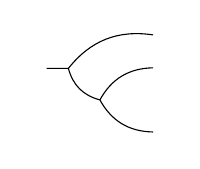
\begin{tikzpicture}[scale=0.8]
	\path (0,0) node (X) {} 
	++ (0.5,0) coordinate (copy0)
	+ (1.5,0.5) node (X1) {}
	++ (0.5,-0.5) coordinate (copy1)
	+(1,0.5) node (X2) {}
	+(1,-0.5) node (X3) {};
	\draw (X) -- (copy0) to [bend left] (X1) (copy0) to [bend right] (copy1) to [bend left] (X2) (copy1) to [bend right] (X3);
	\end{tikzpicture}
	=
	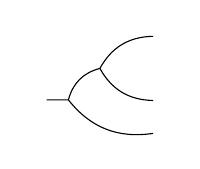
\begin{tikzpicture}[scale=0.8]
	\path (0,0) node (X) {} 
	++ (0.5,0) coordinate (copy0)
	+ (1.5,-0.5) node (X1) {}
	++ (0.5,0.5) coordinate (copy1)
	+(1,0.5) node (X2) {}
	+(1,-0.5) node (X3) {};
	\draw (X) -- (copy0) to [bend right] (X1) (copy0) to [bend left] (copy1) to [bend left] (X2) (copy1) to [bend right] (X3);
	\end{tikzpicture}
	:=
	\begin{tikzpicture}[scale=0.8]
	\path (0,0) node (X) {} 
	++ (0.5,0) coordinate (copy0)
	+ (1,0.5) node (X1) {}
	+(1,0) node (X2) {}
	+(1,-0.5) node (X3) {};
	\draw (X) -- (copy0) to [bend left] (X1) (copy0) to (X2) (copy0) to [bend right] (X3);
	\end{tikzpicture}\label{eq:ccom1}
\end{align}

\begin{align}
	\begin{tikzpicture}[scale=0.8]
	\path (0,0) node (X) {}
	++(0.5,0) coordinate (copy0)
	+ (1,0.5) node (S) {}
	+(1,-0.5) node (X1) {};
	\draw (X) -- (copy0) to [bend right] (X1);
	\draw[-{Rays [n=8]}] (copy0) to [bend left] (S);
	\end{tikzpicture}
	= 
	\begin{tikzpicture}[scale=0.8]
	\path (0,0) node (X) {}
	++(0.5,0) coordinate (copy0)
	+ (1,-0.5) node (S) {}
	+(1,0.5) node (X1) {};
	\draw (X) -- (copy0) to [bend left] (X1);
	\draw[-{Rays [n=8]}] (copy0) to [bend right] (S);
	\end{tikzpicture}
	=
	\begin{tikzpicture}[scale=0.8]
	\path (0,0) node (X) {}
	++ (1,0) node (X1) {};
	\draw (X) -- (X1);
	\end{tikzpicture}\label{eq:ccom2}
\end{align}

\begin{align}
	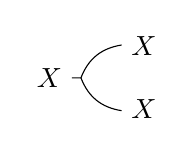
\begin{tikzpicture}[scale=0.8]
	\path (0,0) node (X) {$\RV{X}$}
	++(0.5,0) coordinate (copy0)
	+ (1,0.5) node (X2) {$\RV{X}$}
	+(1,-0.5) node (X1) {$\RV{X}$};
	\draw (X) -- (copy0) to [bend right] (X1);
	\draw (copy0) to [bend left] (X2);
	\end{tikzpicture}
=
	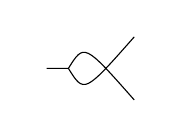
\begin{tikzpicture}[scale=0.8]
	\path (0,0) node (X) {}
	++(0.5,0) coordinate (copy0)
	+ (1.2,0.5) node (X2) {}
	+(1.2,-0.5) node (X1) {};
	\draw (X) -- (copy0) .. controls (0.75,0.4) .. (X1.west);
	\draw (copy0) .. controls (0.75,-0.4) .. (X2.west);
	\end{tikzpicture}
\label{eq:ccom3}
\end{align}

The discard map $\stopper{0.2}$ can ``fall through'' any Markov kernel:

\begin{align}
\begin{tikzpicture}
\path (0,0) node (X) {}
++(0.7,0) node[kernel] (A) {$\kernel{A}$}
++(0.7,0) node (S) {};
\draw (X) -- (A);
\draw[-{Rays [n=8]}] (A) -- (S);
\end{tikzpicture}
= 
\begin{tikzpicture}
\path (0,0) node (X) {}
++(0.7,0) node (S) {};
\draw[-{Rays [n=8]}] (X) -- (S);
\end{tikzpicture}\label{eq:termobj1}
\end{align}

Combining \ref{eq:ccom2} and \ref{eq:termobj1} we can derive the following: integrating $\kernel{A}:X\to \Delta(\mathcal{Y})$ with respect to $\mu\in\Delta(\mathcal{X})$ and then discarding the output of $\kernel{A}$ leaves us with $\mu$:

\begin{align}
\begin{tikzpicture}
\path (0,0) node[dist] (mu) {$\mu$}
++ (1,0) coordinate (copy0)
+ (1.4,0.5) node (X) {}
++ (0.7,-0.5) node[kernel] (A) {$\kernel{A}$}
++(0.7,0) node (Y) {};
\draw (mu)--(copy0);
\draw (copy0) to [bend left] (X);
\draw[-{Rays [n=8]}] (copy0) to [bend right] (A) (A) -- (Y);
\end{tikzpicture}
= 
\begin{tikzpicture}
\path (0,0) node[dist] (mu) {$\mu$}
++ (1,0) coordinate (copy0)
+ (1.2,0.5) node (X) {}
++ (0.4,-0.3) coordinate (A)
++(0.1,0) node (Y) {};
\draw (mu)--(copy0);
\draw (copy0) to [bend left] (X);
\draw[-{Rays [n=8]}] (copy0) to [bend right] (A) (A) -- (Y);
\end{tikzpicture}
=
\begin{tikzpicture}
\path (0,0) node[dist] (mu) {$\mu$}
++ (1,0) node (X) {};
\draw (mu)--(X);
\end{tikzpicture}
\end{align}

In elementary notation, this is equivalent to the fact that, for all $B\in \mathcal{X}$, $\int_B \kernel{A}(x;B)d\mu(x) = \mu(B)$.

The following additional properties hold for $\stopper{0.2}$ and $\splitter{0.1}$:

\begin{align}
\begin{tikzpicture}
\path (0,0) node (XY) {$X\times Y$}
++ (1.5,0) node (Z) {};
\draw[-{Rays [n=8]}] (XY) -- (Z);
\end{tikzpicture} &=
\begin{tikzpicture}
\path (0,0) node (X) {$X$} 
++ (1,0) node (X1) {}
(0,-0.3) node (Y) {$Y$}
++ (1,0) node (Y1) {};
\draw[-{Rays [n=8]}] (X) -- (X1);
\draw[-{Rays [n=8]}] (Y) -- (Y1);
\end{tikzpicture}
\end{align}
\begin{align}
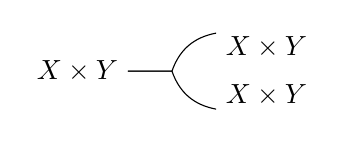
\begin{tikzpicture}
\path (0,0) node (XY) {$X\times Y$}
++ (1.2,0) coordinate (copy0)
++(1.2,0.3) node (XY1) {$X \times Y$}
++(0,-0.6) node (XY2) {$X\times Y$};
\draw (XY) -- (copy0) to [bend left] (XY1);
\draw (XY) -- (copy0) to [bend right] (XY2);
\end{tikzpicture} &=
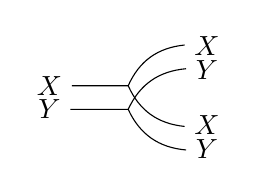
\begin{tikzpicture}
\path (0,0) node (XY) {$X$}
++ (1.,0) coordinate (copy0)
++(1.,0.5) node (XY1) {$X$}
++(0,-1) node (XY2) {$X$}
(0,-0.3) node (F) {$Y$}
++(1.,0) coordinate (copy1)
++(1.,0.5) node (F1) {$Y$}
++(0,-1) node (F2) {$Y$};
\draw (XY) -- (copy0) to [bend left] (XY1);
\draw (copy0) to [bend right] (XY2);
\draw (F) -- (copy1) to [bend left] (F1);
\draw (copy1) to [bend right] (F2);
\end{tikzpicture}
\end{align}

A key fact that \emph{does not} hold in general is

\begin{align}
 \begin{tikzpicture}
\path (0,0) node (E) {}
++ (0.7,0) node[kernel] (A) {$\kernel{A}$}
++(0.7,0) coordinate (copy0)
++(0.5,0.3) node (F1) {}
+(0,-0.6) node (F2) {};
\draw (E) -- (A) -- (copy0) to [bend left] (F1);
\draw (copy0) to [bend right] (F2);
\end{tikzpicture} 
=
\begin{tikzpicture}
\path (0,0) node (E) {}
++(0.5,0) coordinate (copy0)
++(0.7,0.3) node[kernel] (A1) {$\kernel{A}$}
+(0,-0.6) node[kernel] (A2) {$\kernel{A}$}
++(0.75,0) node (F1) {}
+(0,-0.6) node (F2) {};
\draw (E) -- (copy0) to [bend left] (A1) (A1) -- (F1);
\draw (copy0) to [bend right] (A2) (A2) -- (F2);
\end{tikzpicture}
\label{eq:copy_commutes}
\end{align}

In fact, it holds only when $\kernel{A}$ is a \emph{deterministic} kernel.

\begin{definition}[Deterministic Markov kernel]
A \emph{deterministic} Markov kernel $\kernel{A}:E\to \Delta(\mathcal{F})$ is a kernel such that $\kernel{A}_x(B)\in\{0,1\}$ for all $x\in E$, $B\in\mathcal{F}$.
\end{definition}

\begin{theorem}[Copy map commutes for deterministic kernels \citep{fong_causal_2013}]
Equation \ref{eq:copy_commutes} holds iff $\kernel{A}$ is deterministic.
\end{theorem}

\subsubsection{Examples}

Given $\mu\in\Delta(X),\kernel{K}:X\to \Delta(Y)$, $A\in \mathcal{X}$ and $B\in\mathcal{Y}$:

\begin{align}
&A\times B\mapsto \int_A \kernel{K}(x;B)d\mu(x)\\ &\equiv \\\mu 
&\splitter{0.1}(\textbf{Id}_X\otimes \kernel{K})\\ &\equiv \\
&\begin{tikzpicture}
\path (0,0) node[dist] (mu) {$\mu$}
++ (1,0) coordinate (copy0)
+ (1.2,0.5) node (X) {$X$}
++ (0.5,-0.5) node[kernel] (A) {$\kernel{K}$}
++(0.7,0) node (Y) {$Y$};
\draw (mu)--(copy0);
\draw (copy0) to [bend left] (X);
\draw (copy0) to [bend right] (A) (A) -- (Y);
\end{tikzpicture}\label{eq:joint_measure}
\end{align}

\citet{cho_disintegration_2019} calls this operation ``integrating $\kernel{K}$ with respect to $\mu$''.

Given $\nu\in \Delta(\sigalg{X}\otimes\sigalg{Y})$, define the marginal $\nu^{\RV{Y}}\in \Delta(\mathcal{Y}):B\mapsto \mu(X\times B)$ for $B\in \mathcal{Y}$. Say that $\nu^{\RV{Y}}$ is obtained by marginalising over ``$X$'' (a notion that can be made more precise by assigning names to wires). Then

\begin{align}
	\nu(\stopper{0.25}\otimes \mathrm{Id}^Y) &= \begin{tikzpicture}
		\path (0,0) node[dist] (nu) {$\nu$}
		++ (0.7,-0.15) node (X) {$Y$}
		+(0,0.3) node (Y) {};
		\draw ($(nu.east)+(0,-0.15)$) -- (X);
		\draw[-{Rays[n=8]}] ($(nu.east)+(0,0.15)$) -- (Y);
	\end{tikzpicture}\\
	\nu(\stopper{0.25}\otimes \mathrm{Id}^Y)(B) &:= \nu(\stopper{0.25}\otimes \mathrm{Id}^Y)(B\times\{*\})\\
												&=\int_{X\times Y} \mathrm{Id}^Y_y(B) \stopper{0.2}_x(\{*\}) d\nu(x,y)\\
	&= \int_{X\times Y} \delta_y(B) \delta_*(\{*\}) d\nu(x,y)\\
	&= \int_{X\times B} d\nu(x,y)\\
	&= \nu(X\times B)\\
	&= \nu^{\RV{Y}}(B)
\end{align}

Thus the action of the erasing wire ``$X$'' is equivalent to marginalising over ``$X$''.

Consider the result of marginalising \ref{eq:joint_measure} over ``$X$'':
\begin{align}
  \nu^Y (B) &= \begin{tikzpicture}
\path (0,0) node[dist] (mu) {$\mu$}
++ (1,0) coordinate (copy0)
+ (1.2,0.5) node (X) {}
++ (0.5,-0.5) node[kernel] (A) {$\kernel{A}$}
++(0.7,0) node (Y) {$Y$};
\draw (mu)--(copy0);
\draw[-{Rays [n=8]}] (copy0) to [bend left] (X);
\draw (copy0) to [bend right] (A) (A) -- (Y);
\end{tikzpicture} \\
 &= \begin{tikzpicture}
\path (0,0) node[dist] (mu) {$\mu$} ++ (1,0) node[kernel] (A) {$\kernel{A}$} ++ (0.7,0) node (Y) {$Y$}; \draw (mu) -- (A) -- (Y);
\end{tikzpicture} \label{eq:marginalisation_graph}
\end{align}

\subsection{Random Variables}\label{ssec:random_variables}

The summary of this section is:
\begin{itemize}
\item Random variables are usually defined as measurable functions on a \emph{probability space}
\item It's possible to define them as measurable functions on a \emph{Markov kernel space} instead
\item It is useful to label wires with random variable names instead of names of spaces
\end{itemize}

Probability theory is primarily concerned with the behaviour of \emph{random variables}. This behaviour can be analysed via a collection of probability measures and Markov kernels representing joint, marginal and conditional distributions of random variables of interest. In the framework developed by Kolmogorov, this collection of joint, marginal and conditional distributions is modeled by a single underlying \emph{probability space}, and random variables by measurable functions on the probability space. 

We use the same approach here, with a couple of additions. We are interested in variables whose outcomes depend both on random processes and decisions. Suppose that given a particular distribution over decision variables, a probability distribution over the decision variables and random variables is obtained. Such a model is described by a Markov kernel rather than a probability distribution. We therefore investigate \emph{Markov kernel spaces}.

In the graphical notation that we are using, random variables can be thought of as a means of assigning unambiguous names to each wire in a set of diagrams. In order to do this, it is necessary to suppose that all diagrams in the set describe properties of an \emph{ambient Markov kernel} or \emph{ambient probability measure}. Consider the following example with the ambient probability measure $\mu\in\Delta(\mathcal{X}\otimes\mathcal{X})$. Suppose we have a Markov kernel $\kernel{K}:X\to \Delta(\mathcal{X})$ such that the following holds:

\begin{align}
\begin{tikzpicture}
\path (0,0) node[dist] (m) {$\mu$}
++ (0.7,0.15) node (E) {$X$}
++ (0,-0.3) node (F) {$X$};
\draw ($(m.east) + (0,0.15)$) -- (E);
\draw ($(m.east) + (0,-0.15)$) -- (F);
\end{tikzpicture} = \begin{tikzpicture}
\path (0,0) node[dist] (m) {$\mu$}
++ (0.7,0.15) coordinate (copy0)
+(0,-0.3) node (Fs) {}
++ (1.2,0) node (E) {$X$}
++(-0.7,-0.3) node[kernel] (K) {$\kernel{K}$}
++(0.7,0) node (F) {$X$};
\draw ($(m.east) + (0,0.15)$) -- (E);
\draw (copy0) to [bend right] (K) (K) -- (F);
\draw[-{Rays [n=8]}] ($(m.east) + (0,-0.15)$) -- (Fs);
\end{tikzpicture}\label{eq:disint_example}
\end{align}

Suppose that we also assign the names $\RV{X}_1$ to the upper output wire and $\RV{X}_2$ to the lower output wire in the diagram of $\mu$:

\begin{align}
\begin{tikzpicture}
\path (0,0) node[dist] (m) {$\mu$}
++ (0.7,0.15) node (E) {$\RV{X}_1$}
++ (0,-0.3) node (F) {$\RV{X}_2$};
\draw ($(m.east) + (0,0.15)$) -- (E);
\draw ($(m.east) + (0,-0.15)$) -- (F);
\end{tikzpicture}
\end{align}

Then it seems sensible to call $\kernel{K}$ ``the probability of $\RV{X}_2$ given $\RV{X}_1$''. We will make this precise, and it will match the usual notion of the probability of one variable given another (see \citet{cinlar_probability_2011} for a definition of this usual notion). 

\begin{definition}[Probability space, Markov kernel space]\label{def:kernel_space}
A \emph{Markov kernel space} $(\kernel{K},(D,\mathcal{D}),(\Omega,\mathcal{F}))$ is a Markov kernel $\kernel{K}:D\to \Delta(\mathcal{D}\otimes\mathcal{F})$, called the \emph{ambient kernel}, along with the sample space $(\Omega,\mathcal{F})$ and the domain $(D,\mathcal{D})$. We suppose that $\kernel{K}$ is such that there exists a \emph{fundamental kernel} $\kernel{K}_0$ satisfying

\begin{align}
\prob{K} := \begin{tikzpicture}
\path (0,0) node (O) {}
++(0.5,0) coordinate (copy0)
++ (0.5,0) node[kernel] (m) {$\kernel{K}_0$}
++ (0.7,0.) node (E) {}
++(0,-0.45) node (G) {};
\draw (O) -- (m) -- (E);
\draw (copy0) to [bend right] (G);
\end{tikzpicture}
\end{align}

For brevity, we will omit the $\sigma$-algebras in further definitions of Markov kernel spaces: $(\kernel{K},D,\Omega)$.

A \emph{probability space} $(\prob{P},\Omega,\mathcal{F})$ is a probability measure $\prob{P}:\Delta(\Omega)$, which we call the \emph{ambient measure}, along with the \emph{sample space} $\Omega$ and the \emph{events} $\mathcal{F}$. A probability space is equivalent to a Markov kernel space with domain $D=\{*\}$ - note that $\Omega\times \{*\}\cong \Omega$.
\end{definition}

\begin{definition}[Random variable]\label{def:random_variable}
Given a Markov kernel space $(\kernel{K},D,\Omega)$, a random variable $\RV{X}$ is a measurable function $\Omega\times D\to E$ for arbitrary measurable $E$.
\end{definition}

\begin{definition}[Domain variable]\label{def:domain_variable}
Given a Markov kernel space $(\kernel{K},D,\Omega)$, the \emph{domain variable} $\RV{D}:\Omega\times D\to D$ is the distinguished random variable $\RV{D}:(x,d)\mapsto d$.
\end{definition}

Unlike random variables on probability spaces, random variables on Markov kernel spaces do not generally have unique marginal distributions. An analogous operation of \emph{marginalisation} can be defined, but the result is generally a Markov kernel. We will define marginalisation via coupled tensor products.

\begin{definition}[Coupled tensor product $\utimes$]\label{def:ctensor}
Given two Markov kernels $\kernel{M}$ and $\kernel{N}$ or functions $f$ and $g$ with shared domain $E$, let $\kernel{M}\utimes\kernel{N}:=\splitter{0.1}(\kernel{M}\otimes\kernel{N})$ and $f\utimes g:=\splitter{0.1}(f\otimes g)$ where these expressions are interpreted using standard product notation. Graphically:

\begin{align}
\kernel{M}\utimes\kernel{N}&:=\begin{tikzpicture}
\path (0,0) node (E) {$E$}
++(0.5,0) coordinate (copy0)
+ (0.5,0.3) node[kernel] (M) {$\kernel{M}$}
+(1.2,0.3) node (X) {$\RV{X}$}
+ (0.5,-0.3) node[kernel] (N) {$\kernel{N}$}
+(1.2,-0.3) node (Y) {$\RV{Y}$};
\draw (E) -- (copy0) to [bend left] (M) (copy0) to [bend right] (N);
\draw (M) -- (X) (N) -- (Y);
\end{tikzpicture}\\
f\utimes g&:= \begin{tikzpicture}[scale=1.2]\path (0,0) node (E) {$E$}
++(0.5,0) coordinate (copy0)
+ (0.5,0.3) node[expectation] (M) {$f$}
+ (0.5,-0.3) node[expectation] (N) {$g$};
\draw (E) -- (copy0) to [bend left] (M) (copy0) to [bend right] (N);
\end{tikzpicture}
\end{align}
The operation denoted by $\utimes$ is associative (Lemma \ref{lem:utimes_assoc}), so we can without ambiguity write $f\utimes g\utimes h=(f\utimes g)\utimes h = f\utimes(g\utimes h)$ for finite groups of functions or Markov kernels sharing a domain. 

The notation $\utimes_{i\in [N]} f_i$ is taken to mean $f_1\utimes f_2\utimes ...\utimes f_N$.
\end{definition}

\begin{lemma}[$\utimes$ is associative]\label{lem:utimes_assoc}
For Markov kernels $\kernel{L}:E\to \delta(\mathcal{F})$, $\kernel{M}:E\to \delta(\mathcal{G})$ and $\kernel{N}:E\to \delta(\mathcal{H})$, $(\kernel{L}\utimes\kernel{M})\utimes\kernel{N}=\kernel{L}\utimes(\kernel{M}\utimes\kernel{N})$.
\end{lemma}

\begin{proof}

\begin{align}
	\kernel{L}\utimes(\kernel{M}\utimes\kernel{N}) &= 
	\begin{tikzpicture}[scale=0.8]
	\path (0,0) node (X) {$E$} 
	++ (0.8,0) coordinate (copy0)
	+ (1.5,0.5) node[kernel] (X1) {$\kernel{L}$} + (2.5,0.5) node (F) {$F$}
	++ (0.5,-0.5) coordinate (copy1)
	+(1,0.3) node[kernel] (X2) {$\kernel{M}$} + (2,0.3) node (G) {$G$}
	+(1,-0.5) node[kernel] (X3) {$\kernel{N}$} + (2,-0.5) node (H) {$H$};
	\draw (X) -- (copy0) to [bend left] (X1) (copy0) to [bend right] (copy1) to [bend left] (X2) (copy1) to [bend right] (X3);
	\draw (X1) -- (F) (X2) -- (G) (X3) -- (H);
	\end{tikzpicture}\\
	&=
	\begin{tikzpicture}[scale=0.8]
	\path (0,0) node (X) {$E$} 
	++ (0.8,0) coordinate (copy0)
	+ (1.5,0.7) node[kernel] (X1) {$\kernel{L}$} + (2.5,0.7) node (F) {$F$}
	+ (0.5,0.3) coordinate (copy1)
	++ (0.5,-0.5) coordinate (next)
	+(1,0.5) node[kernel] (X2) {$\kernel{M}$} + (2,0.5) node (G) {$G$}
	+(1,-0.5) node[kernel] (X3) {$\kernel{N}$} + (2,-0.5) node (H) {$H$};
	\draw (X) -- (copy0) to [bend left] (copy1) (copy0) to [bend right] (X3);
	\draw (copy1) to [bend left] (X1) (copy1) to [bend right] (X2);
	\draw (X1) -- (F) (X2) -- (G) (X3) -- (H);
	\end{tikzpicture}\\
	&= (\kernel{L}\utimes\kernel{M})\utimes\kernel{N}
\end{align}
This follows directly from Equation \ref{eq:ccom1}.
\end{proof}

\begin{definition}[Marginal distribution, marginal kernel]\label{def:marginal_distribution}
Given a probability space $(\prob{P},\Omega,\mathcal{F})$ and the random variable $\RV{X}:\Omega\to G$ the \emph{marginal distribution} of $\RV{X}$ is the probability measure $\prob{P}^{\RV{X}}:= \prob{P}\kernel{F}^{\RV{X}}$.

See Lemma \ref{lem:pushf_funk} for the proof that this matches the usual definition of marginal distribution.

Given a Markov kernel space $(\kernel{K},\Omega,\mathcal{F},D,\mathcal{D})$ and the random variable $\RV{X}:\Omega\to G$, the \emph{marginal kernel} is $\kernel{K}^{\RV{X}|\RV{D}}:=\kernel{K}\kernel{F}^{\RV{X}}$.
\end{definition}

\begin{definition}[Joint distribution, joint kernel]\label{def:joint_distribution}
Given a probability space $(\prob{P},\Omega,\mathcal{F})$ and the random variables $\RV{X}:\Omega\to G$ and $\RV{Y}:\Omega\to H$, the \emph{joint distribution} of $\RV{X}$ and $\RV{Y}$, $\prob{P}^{\RV{X}\RV{Y}}\in \Delta(\mathcal{G}\otimes\mathcal{H})$, is the marginal distribution of $\RV{X}\utimes\RV{Y}$. That is, $\prob{P}^{\RV{X}\RV{Y}}:=\prob{P} \kernel{F}^{\RV{X}\utimes\RV{Y}}$

This is identical to the definition in \citet{cinlar_probability_2011} if we note that the random variable $(\RV{X},\RV{Y}):\omega\mapsto (\RV{X}(\omega),\RV{Y}(\omega))$ (\c{C}inlar's definition) is precisely the same thing as $\RV{X}\utimes\RV{Y}$.

Analogously, the joint kernel $\kernel{K}^{\RV{X}\RV{Y}|\RV{D}}$ is the product $\kernel{K}\kernel{F}^{\RV{X}\utimes\RV{Y}}$.
\end{definition}

Joint distributions and kernels have a nice visual representation, as a result of Lemma \ref{lem:jdist_cprod} which follows.

\begin{lemma}[Product marginalisation interchange]\label{lem:jdist_cprod}
Given two functions, the kernel associated with their coupled product is equal to the coupled product of the kernels associated with each function.

Given $\RV{X}:\Omega\to G$ and $\RV{Y}:\Omega\to H$, $\kernel{F}^{\RV{X}\utimes\RV{Y}}=\kernel{F}^\RV{X}\utimes\kernel{F}^\RV{Y}$
\end{lemma}

\begin{proof}
For $a\in \Omega$, $B\in \mathcal{G}$, $C\in \mathcal{H}$,
\begin{align}
\kernel{F}^{\RV{X}\utimes\RV{Y}} (a;B\times C) &= \delta_{\RV{X}(a),\RV{Y}(a)}(B\times C)\\
									   &= \delta_{\RV{X}(a)}(B)\delta_{\RV{Y}(a)}(C)\\
									   &= (\delta_{\RV{X}(a)}\otimes\delta_{\RV{Y}(a)})(B\times C)\\
									   &= \kernel{F}^{\RV{X}}\utimes\kernel{F}^{\RV{Y}}
\end{align}
Equality follows from the monotone class theorem.
\end{proof}

\begin{corollary}\label{corr:rewrite_joint_dist}
Given a Markov kernel space $(\kernel{K}, \Omega, D)$ and random variables $\RV{X}:\Omega\times D\to X$, $\RV{Y}:\Omega\times D\to Y$, the following holds:

\begin{align}
\begin{tikzpicture}
\path (0,0) node (O) {$D$}
++(1,0) node[kernel] (K) {$\kernel{K}^{\RV{X}\RV{Y}|\RV{D}}$}
++ (1,0.15) node (X) {$X$}
+(0,-0.3) node (Y) {$Y$};
\draw (O) -- (K);
\draw ($(K.east) + (0,0.15)$) -- (X);
\draw ($(K.east) + (0,-0.15)$) -- (Y);
\end{tikzpicture}=
\begin{tikzpicture}
\path (0,0) node (O) {$D$}
++ (0.7, 0) node[kernel] (K) {$\kernel{K}$}
++ (0.6,0) coordinate (copy0)
++ (0.4,0.25) node[kernel] (X) {$\kernel{F}^{\RV{X}}$}
+(0,-0.5) node[kernel] (Y) {$\kernel{F}^{\RV{Y}}$}
++(0.7,0) node (Xo) {$X$}
+(0,-0.5) node (Yo) {$Y$};
\draw (O) -- (K) -- (copy0);
\draw (copy0) to [bend left] (X) (X) -- (Xo);
\draw (copy0) to [bend right] (Y) (Y) -- (Yo);
\end{tikzpicture}
\end{align}
\end{corollary}

We will now define wire labels for ``output'' wires.

\begin{definition}[Wire labels - joint kernels]\label{def:wl_jprob}
Suppose we have a Markov kernel space $(\kernel{K},D,\Omega)$, random variables $\RV{X}:\Omega\times D\to X$, $\RV{Y}:\Omega\times D\to Y$ and a Markov kernel $\kernel{L}:D\to \Delta(\mathcal{X}\times\mathcal{Y})$. The following \emph{output labelling} of $\mathbf{L}$:

\begin{align}
\begin{tikzpicture}
\path (0,0) node (A) {$D$}
++ (0.7,0) node[kernel] (m) {$\kernel{L}$}
++ (0.7,0.15) node (E) {\color{blue}$\RV{X}$}
++ (0,-0.3) node (F) {\color{blue}$\RV{Y}$};
\draw (A) -- (m);
\draw ($(m.east) + (0,0.15)$) -- (E);
\draw ($(m.east) + (0,-0.15)$) -- (F);
\end{tikzpicture}
\end{align}

is \emph{valid} iff

\begin{align}
\kernel{L} = \kernel{K}_{\RV{X}\RV{Y}|\RV{D}}\label{eq:labels_express_joint}
\end{align}

and

\begin{align}
\begin{tikzpicture}
\path (0,0) node (A) {$D$}
++ (1,0) node[kernel] (m) {$\kernel{L}$}
++ (1,0.15) node (E) {\color{blue}$\RV{X}$}
++ (0,-0.3) node (F) {};
\draw (A) -- (m) ($(m.east) + (0,0.15)$) -- (E);
\draw[-{Rays [n=8]}] ($(m.east) + (0,-0.15)$) -- (F);
\end{tikzpicture} = \kernel{K}^{\RV{X}|\RV{D}}\label{eq:labels_express_marginal_upper}
\end{align}

and

\begin{align}
\begin{tikzpicture}
\path (0,0) node (A) {$D$}
++ (1,0) node[kernel] (m) {$\kernel{L}$}
++ (1,0.15) node (E) {}
++ (0,-0.3) node (F) {\color{blue}$\RV{Y}$};
\draw (A) -- (m);
\draw[-{Rays [n=8]}] ($(m.east) + (0,0.15)$) -- (E);
\draw ($(m.east) + (0,-0.15)$) -- (F);
\end{tikzpicture} = \kernel{K}^{\RV{Y}|\RV{D}}\label{eq:labels_express_marginal_lower}
\end{align}

The second and third conditions are nontrivial: suppose $\RV{X}$ takes values in some product space $Range(\RV{X}) = W\times Z$, and $\RV{Y}$ takes values in $Y$. Then we could have $\kernel{L}=\kernel{K}^{\RV{X}\RV{Y}|\RV{D}}$ and draw the diagram

\begin{align}
\begin{tikzpicture}
\path (0,0) node (A) {$D$}
++ (0.7,0) node[kernel] (m) {$\kernel{L}$}
++ (1,0.15) node (E) {$W$}
++ (0.3,-0.3) node (F) {$Z\times Y$};
\draw (A) -- (m);
\draw ($(m.east) + (0,0.15)$) -- (E);
\draw ($(m.east) + (0,-0.15)$) -- (F);
\end{tikzpicture}\label{eq:cannot_marginalise}
\end{align}

For \emph{this} diagram, properties \ref{eq:labels_express_marginal_upper} and \ref{eq:labels_express_marginal_lower} do not hold, even though \ref{eq:labels_express_joint} does.

\end{definition}

\begin{lemma}[Output label assignments exist]
Given Markov kernel space $(\kernel{K},D,\Omega)$, random variables $\RV{X}:\Omega\times D\to X$ and $\RV{Y}:\Omega\times D\to Y$ then there exists a diagram of $\kernel{L}:=\kernel{K}^{\RV{X}\RV{Y}|\RV{D}}$ with a valid output labelling assigning ${\color{blue}\RV{X}}$ and ${\color{blue}\RV{Y}}$ to the output wires.
\end{lemma}

\begin{proof}
By definition, $\kernel{L}$ has signature $D\to \Delta(\mathcal{X}\otimes\mathcal{Y})$. Thus, by the rule that tensor product spaces can be represented by parallel wires, we can draw

\begin{align}
\begin{tikzpicture}
\path (0,0) node (A) {$D$}
++ (0.7,0) node[kernel] (m) {$\kernel{L}$}
++ (0.7,0.15) node (E) {$X$}
++ (0,-0.3) node (F) {$Y$};
\draw (A) -- (m);
\draw ($(m.east) + (0,0.15)$) -- (E);
\draw ($(m.east) + (0,-0.15)$) -- (F);
\end{tikzpicture}
\end{align}

By Corollary \ref{corr:rewrite_joint_dist}, we have

\begin{align}
\begin{tikzpicture}
\path (0,0) node (A) {$D$}
++ (0.7,0) node[kernel] (m) {$\kernel{L}$}
++ (0.7,0.15) node (E) {$X$}
++ (0,-0.3) node (F) {$Y$};
\draw (A) -- (m);
\draw ($(m.east) + (0,0.15)$) -- (E);
\draw ($(m.east) + (0,-0.15)$) -- (F);
\end{tikzpicture} = \begin{tikzpicture}
\path (0,0) node (O) {$D$}
++ (0.7, 0) node[kernel] (K) {$\kernel{K}$}
++ (0.6,0) coordinate (copy0)
++ (0.4,0.25) node[kernel] (X) {$\kernel{F}^{\RV{X}}$}
+(0,-0.5) node[kernel] (Y) {$\kernel{F}^{\RV{Y}}$}
++(0.7,0) node (Xo) {$X$}
+(0,-0.5) node (Yo) {$Y$};
\draw (O) -- (K) -- (copy0);
\draw (copy0) to [bend left] (X) (X) -- (Xo);
\draw (copy0) to [bend right] (Y) (Y) -- (Yo);
\end{tikzpicture}
\end{align}

Therefore 

\begin{align}
\begin{tikzpicture}
\path (0,0) node (O) {$D$}
++ (0.7, 0) node[kernel] (K) {$\kernel{K}$}
++ (0.6,0) coordinate (copy0)
++ (0.4,0.25) node[kernel] (X) {$\kernel{F}^{\RV{X}}$}
+(0,-0.5) node[kernel] (Y) {$\kernel{F}^{\RV{Y}}$}
++(0.7,0) node (Xo) {$X$}
+(0,-0.5) node (Yo) {};
\draw (O) -- (K) -- (copy0);
\draw (copy0) to [bend left] (X) (X) -- (Xo);
\draw[-{Rays[n=8]}] (copy0) to [bend right] (Y) (Y) -- (Yo);
\end{tikzpicture} &= \kernel{K}\kernel{F}^{\RV{X}}\\
				 &= \kernel{K}^{\RV{X}|\RV{D}}
\end{align}

\begin{align}
\begin{tikzpicture}
\path (0,0) node (O) {$D$}
++ (0.7, 0) node[kernel] (K) {$\kernel{K}$}
++ (0.6,0) coordinate (copy0)
++ (0.4,0.25) node[kernel] (X) {$\kernel{F}^{\RV{X}}$}
+(0,-0.5) node[kernel] (Y) {$\kernel{F}^{\RV{Y}}$}
++(0.7,0) node (Xo) {}
+(0,-0.5) node (Yo) {$Y$};
\draw (O) -- (K) -- (copy0);
\draw[-{Rays[n=8]}] (copy0) to [bend left] (X) (X) -- (Xo);
\draw (copy0) to [bend right] (Y) (Y) -- (Yo);
\end{tikzpicture} &= \kernel{K}\kernel{F}^{\RV{Y}}\\
				 &= \kernel{K}^{\RV{Y}|\RV{D}}
\end{align}
\end{proof}

In all further work, wire labels will be used without special colouring.

\begin{definition}[Disintegration]\label{def:disintegration}
Given a probability space $(\prob{P},\Omega,\mathcal{F})$, and random variables $\RV{X}$ and $\RV{Y}$, we say that $\kernel{M}:E\to \Delta(\mathcal{F})$ is a \emph{$\RV{Y}$ on $\RV{X}$ disintegration} of $\prob{P}$ iff
\begin{align}
\begin{tikzpicture}
\path (0,0) node[dist] (m) {$\prob{P}^{\RV{X}\RV{Y}}$}
++ (1,0.15) node (E) {$\RV{X}$}
++ (0,-0.3) node (F) {$\RV{Y}$};
\draw ($(m.east) + (0,0.15)$) -- (E);
\draw ($(m.east) + (0,-0.15)$) -- (F);
\end{tikzpicture} = \begin{tikzpicture}
\path (0,0) node[dist] (m) {$\prob{P}^{\RV{X}}$}
++ (0.7,0.15) coordinate (copy0)
+(0.2,-0.3) node (T) {}
++ (1.2,0) node (E) {$\RV{X}$}
++(-0.7,-0.3) node[kernel] (K) {$\kernel{M}$}
++(0.7,0) node (F) {$\RV{Y}$};
\draw ($(m.east) + (0,0.15)$) -- (E);
\draw (copy0) to [bend right] (K) (K) -- (F);
\draw[-{Rays [n=8]}] ($(m.east) + (0,-0.15)$) -- (T);
\end{tikzpicture}\label{eq:ordinary_disint}
\end{align}
$\kernel{M}$ is a version of $\prob{P}^{\RV{Y}|\RV{X}}$, ``the probability of $\RV{Y}$ given $\RV{X}$''. Let $\prob{P}^{\{\RV{Y}|\RV{X}\}}$ be the set of all kernels that satisfy \ref{eq:ordinary_disint} and $\prob{P}^{\RV{Y}|\RV{X}}$ an arbitrary member of $\prob{P}^{\RV{Y}|\RV{X}}$.

Given a Markov kernel space $(\kernel{K},D,\Omega)$ and random variables $\RV{X}:\Omega\times D\to X$, $\RV{Y}:\Omega\times D\to Y$, $\kernel{M}:D\times E\to \Delta(\mathcal{F})$ is a \emph{$\RV{Y}$ on $\RV{DX}$ disintegration} of $\kernel{K}^{\RV{YX}|\RV{D}}$ iff

\begin{align}
\begin{tikzpicture}
\path (0,0) node (O) {}
++ (1,0) node[kernel] (m) {$\kernel{K}^{\RV{YX}|\RV{D}}$}
++ (1,0.15) node (E) {$\RV{X}$}
++ (0,-0.3) node (F) {$\RV{Y}$};
\draw (O) -- (m) ($(m.east) + (0,0.15)$) -- (E);
\draw ($(m.east) + (0,-0.15)$) -- (F);
\end{tikzpicture} = \begin{tikzpicture}
\path (0,0) node (O) {}
++ (0.3,0) coordinate (copy1)
++ (1,0) node[kernel] (m) {$\kernel{K}^{\RV{YX}|\RV{D}}$}
++ (1,0.15) coordinate (copy0)
+(0.2,-0.3) node (T) {}
++ (1.2,0) node (E) {$\RV{X}$}
++(-0.7,-0.3) node[kernel] (K) {$\kernel{M}$}
++(0.7,0) node (F) {$\RV{Y}$};
\draw (O) -- (m) ($(m.east) + (0,0.15)$) -- (E);
\draw (copy0) to [bend right] (K) (K) -- (F);
\draw (copy1) to [out=290,in=180] ($(K.west) + (0,-0.15)$);
\draw[-{Rays [n=8]}] ($(m.east) + (0,-0.15)$) -- (T);
\end{tikzpicture}\label{eq:def_k_disint}
\end{align}

Write $\kernel{K}^{\{\RV{Y}|\RV{XD}\}}$ for the set of kernels satisfying \ref{eq:def_k_disint} and $\kernel{K}^{\RV{Y}|\RV{XD}}$ for an arbitrary member of $\kernel{K}^{\{\RV{Y}|\RV{XD}\}}$.
\end{definition}

\begin{definition}[Wire labels -- input]\label{def:wl_disint}

An input wire is \emph{connected} to an output wire if it is possible to trace a path from the start of the input wire to the end of the output wire without passing through any boxes, erase maps or right facing triangles.

If an input wire is connected to an output wire and that output wire has a valid label $\RV{X}$, then it is valid to label the input wire with $\RV{X}$.

For example, if the following are valid output labels with respect to $(\prob{P},\Omega)$:

\begin{align}
\begin{tikzpicture}
\path (0,0) node (A) {}
++ (0.7,0) coordinate (copy0)
++ (0.7,0) node[kernel] (m) {$\kernel{L}$}
++ (0.7,0) node (E) {\color{blue}$\RV{X}$}
++ (0,-0.3) node (F) {\color{blue}$\RV{Y}$};
\draw (A) -- (m) -- (E);
\draw (copy0) to [out=-60,in=180] (F);
\end{tikzpicture}\label{dia:kernel_l}
\end{align}

i.e. if $\kernel{L}\in \prob{P}^{\{\RV{X}\RV{Y}|\RV{Y}\}}$, then the following is a valid input label:


\begin{align}
\begin{tikzpicture}
\path (0,0) node (A) {\color{blue}$\RV{Y}$}
++ (0.7,0) coordinate (copy0)
++ (0.7,0) node[kernel] (m) {$\kernel{L}$}
++ (0.7,0) node (E) {\color{blue}$\RV{X}$}
++ (0,-0.3) node (F) {\color{blue}$\RV{Y}$};
\draw (A) -- (m) -- (E);
\draw (copy0) to [out=-60,in=180] (F);
\end{tikzpicture}
\end{align}

An input wire in a diagram for $\kernel{M}$ may be labeled $\RV{X}$ \emph{if and only if} copy and identity maps can be inserted to yield a diagram in which the input wire labeled $\RV{X}$ is connected to an output wire with valid label $\RV{X}$.

So, if $\kernel{M}\in \prob{P}^{\{\RV{X}|\RV{Y}\}}$, then it is straightforward to show that

\begin{align}
\begin{tikzpicture}
\path (0,0) node (A) {}
++ (0.7,0) coordinate (copy0)
++ (0.7,0) node[kernel] (m) {$\kernel{M}$}
++ (0.7,0) node (E) {\color{blue}$\RV{X}$}
++ (0,-0.3) node (F) {\color{blue}$\RV{Y}$};
\draw (A) -- (m) -- (E);
\draw (copy0) to [out=-60,in=180] (F);
\end{tikzpicture} \in \prob{P}^{\{\RV{X}\RV{Y}|\RV{Y}\}} \label{eq:const_from_m}
\end{align}

and hence the output labels are valid. Diagram \ref{eq:const_from_m} is constructed by taking the product of the copy map with $\kernel{M}\otimes\textbf{Id}$. Thus it is valid to label $\kernel{M}$ with

\begin{align}
\begin{tikzpicture}
\path (0,0) node (A) {\color{blue}$\RV{Y}$}
++ (0.7,0) node[kernel] (m) {$\kernel{M}$}
++ (0.7,0) node (E) {\color{blue}$\RV{X}$};
\draw (A) -- (m) -- (E);
\end{tikzpicture}
\end{align}
\end{definition}

\begin{lemma}[Labeling of disintegrations]
Given a kernel space $(\kernel{K},D,\Omega)$, random variables $\RV{X}$ and $\RV{Y}$, domain variable $\RV{D}$ and disintegration $\kernel{L}\in \kernel{K}^{\{\RV{Y}|\RV{X}\RV{D}\}}$, there is a diagram of $\kernel{L}$ with valid input labels ${\color{blue} \RV{X}}$ and ${\color{blue} \RV{D}}$ and valid output label ${\color{blue} \RV{Y}}$.
\end{lemma}

\begin{proof}
Note that for any variable $\RV{W}:\Omega\times D\to W$ and the domain variable $\RV{D}:\Omega\times D\to D$ we have by definition of $\kernel{K}$:
\begin{align}
\begin{tikzpicture}
\path (0,0) node (O) {}
++ (1,0) node[kernel] (m) {$\kernel{K}^{\RV{WD}|\RV{D}}$}
++ (1,0.15) node (E) {$\RV{W}$}
++ (0,-0.3) node (F) {$\RV{D}$};
\draw (O) -- (m) ($(m.east) + (0,0.15)$) -- (E);
\draw ($(m.east) + (0,-0.15)$) -- (F);
\end{tikzpicture} &= \begin{tikzpicture}
\path (0,0) node (O) {}
++ (0.3,0) coordinate (copy1)
++ (1,0) node[kernel] (m) {$\kernel{K}_{0}$}
++ (0.7,0) coordinate (copy0)
+ (0,-0.5) coordinate (copy2)
++ (0.7,0.3) node[kernel] (Fx) {$\kernel{F}^\RV{W}$}
++(0,-0.8) node[kernel] (Fd) {$\kernel{F}^{\RV{D}}$}
++(0.7,0) node (D) {$\RV{D}$}
++ (0,0.8) node (X) {$\RV{W}$};
\draw (O) -- (m) -- (copy0);
\draw (copy0) to [bend left] ($(Fx.west)+(0,0.1)$) (copy0) to [bend right] ($(Fd.west)+(0,0.1)$);
\draw (copy1) to [out=290,in=180] (copy2);
\draw (copy2) to [bend left] ($(Fx.west)+(0,-0.1)$) (copy2) to [bend right] ($(Fd.west)+(0,-0.1)$);
\draw (Fx) -- (X) (Fd) -- (D);
\end{tikzpicture}\\
&= \begin{tikzpicture}
\path (0,0) node (O) {}
++ (0.3,0) coordinate (copy1)
++ (1,0) node[kernel] (m) {$\kernel{K}_{0}$}
++ (0.7,0) coordinate (copy0)
+ (0,-0.5) coordinate (copy2)
++ (0.7,0.3) node[kernel] (Fx) {$\kernel{F}^\RV{W}$}
++(0,-0.8) coordinate (Fd)
++(0.7,0) node (D) {$\RV{D}$}
++ (0,0.8) node (X) {$\RV{W}$};
\draw (O) -- (m) -- (copy0);
\draw (copy0) to [bend left] ($(Fx.west)+(0,0.1)$);
\draw (copy1) to [out=290,in=180] (copy2) -- (D);
\draw (copy2) to [bend left] ($(Fx.west)+(0,-0.1)$);
\draw (Fx) -- (X) (Fd) -- (D);
\end{tikzpicture}\\
&= \begin{tikzpicture}
\path (0,0) node (O) {}
++ (0.3,0) coordinate (copy1)
+ (0.2,0) coordinate (copy3)
++ (1,0) node[kernel] (m) {$\kernel{K}_{0}$}
++ (0.7,0) coordinate (copy0)
+ (0,-0.5) coordinate (copy2)
++ (0.7,-0.1) node[kernel] (Fx) {$\kernel{F}^\RV{W}$}
++(0,-0.5) coordinate (Fd)
++(0.7,0) node (D) {$\RV{D}$}
++ (0,0.5) node (X) {$\RV{W}$};
\draw (O) -- (m);
\draw (m) to [out=0,in=180]  ($(Fx.west)+(0,0.1)$);
\draw (copy1) to [out=290,in=180] (D);
\draw (copy3) to [out=290,in=180] ($(Fx.west)+(0,-0.1)$);
\draw (Fx) -- (X);
\end{tikzpicture}\\
&= \begin{tikzpicture}
\path (0,0) node (O) {}
++ (0.3,0) coordinate (copy1)
++ (1,0) node[kernel] (m) {$\kernel{K}$}
++ (0.7,0) coordinate (copy0)
+ (0,-0.5) coordinate (copy2)
++ (0.7,-0.) node[kernel] (Fx) {$\kernel{F}^\RV{W}$}
++(0,-0.5) coordinate (Fd)
++(0.7,0) node (D) {$\RV{D}$}
++ (0,0.5) node (X) {$\RV{W}$};
\draw (O) -- (m);
\draw (m) to [out=0,in=180]  ($(Fx.west)+(0,0.0)$);
\draw (copy1) to [out=290,in=180] (D);
\draw (Fx) -- (X);
\end{tikzpicture}\\
&=\begin{tikzpicture}
\path (0,0) node (O) {}
++ (0.3,0) coordinate (copy1)
++ (1,0) node[kernel] (m) {$\kernel{K}^{\RV{W}|\RV{D}}$}
++(0,-0.5) coordinate (Fd)
++(1,0) node (D) {$\RV{D}$}
++ (0,0.5) node (X) {$\RV{W}$};
\draw (O) -- (m) -- (X);
\draw (copy1) to [out=290,in=180] (D);
\end{tikzpicture}
\end{align}
\end{proof}

We use the informal convention of labelling wires in quote marks $``\RV{X}''$ if that wire is ``supposed to'' carry the label $\RV{X}$ but the label may not be valid.

\begin{theorem}[Iterated disintegration]\label{th:iterated_disint}
Given a kernel space $(\kernel{K},D,\Omega)$, random variables $\RV{X}$, $\RV{Y}$ and $\RV{Z}$ and domain variable $\RV{D}$,
\begin{align}
\begin{tikzpicture}
	\path (0,0.15) node (D) {$``\RV{D}''$}
	+ (0,-0.3) node (X) {$``\RV{X}''$}
	++ (.7,-0.15) coordinate (copy0)
	++ (.7,0) node[kernel] (Yxd) {$\kernel{K}^{\RV{Y}|\RV{XD}}$}
	++ (0.7,0) coordinate (copy1)
	++(1.5,0) node[kernel] (Zxyd) {$\kernel{K}^{\RV{Z}|\RV{XYD}}$}
	++(1.5,0) node (Z) {$``\RV{Z}''$}
	+(0,-0.4) node (Y) {$``\RV{Y}''$};
	\draw (D) -- ($(Yxd.west) + (0,0.15)$) (X) -- ($(Yxd.west) + (0,-0.15)$);
	\draw (Yxd) -- (Zxyd);
	\draw ($(copy0) + (0,0.15)$) to [out=90,in=180] ($(Zxyd.west)+(0,0.15)$);
	\draw ($(copy0) + (0,-0.15)$) to [out=-90,in = 180] ($(Zxyd.west)+(0,-0.15)$);
	\draw (copy1) to [out=-90,in=180] (Y) (Zxyd) -- (Z);
\end{tikzpicture}\in \kernel{K}^{\{\RV{ZY}|\RV{XD}\}}
\end{align}

Equivalently, for $d\in D$ and $x\in X$, $A\in \sigalg{Y}$, $B\in\sigalg{Z}$,

\begin{align}
	(d,x;A,B)\mapsto \int_A \kernel{K}^{\RV{Z}|\RV{XYD}}_{(x,y,d)}(B) d\kernel{K}^{\RV{Y}|\RV{XD}}_{(x,d)}(y) \in \kernel{K}^{\{\RV{ZY}|\RV{XD}\}}
\end{align}
\end{theorem}

\begin{proof}
\todo[inline]{write this up}



\end{proof}

The existence of disintegrations of standard measurable probability spaces is well known.

\begin{theorem}[Disintegration existence - probability space]\label{th:disintegration_exist}
Given a probability measure $\mu\in \Delta(\mathcal{X}\otimes \mathcal{Y})$, if $(F,\mathcal{F})$ is standard then a disintegration $\kernel{K}:X\to \Delta(\mathcal{Y})$ exists \citep{cinlar_probability_2011}.
\end{theorem}

In particular, if for all $x\in X$, $\prob{P}^{\RV{X}}(\RV{X}\in\{x\})>0$, then $\prob{P}^{\RV{Y}|\RV{X}}_x(\RV{Y}\in A) = \frac{\prob{P}^{\RV{X}\RV{Y}}(\RV{Y}\in A \And \RV{X}\in \{x\})}{\prob{P}^{\RV{X}}(\RV{X}\in\{x\})}$.

For Markov kernel spaces, we make the simplifying assumption that the domain space $D$ is a discrete space. Given this assumption, there exists a positive definite probability $\mu\in \Delta(\mathcal{D})$. That is, for every $d\in D$, $\mu(\{d\})>0$. Given this assumption, for every Markov kernel space $(\kernel{K},D,\Omega)$ there is a probability space $(\prob{P},\Omega\times D)$ such that $\kernel{K}$ can be uniquely defined as a disintegration of $\prob{P}$. For uncountable $D$, even if it is standard measurable, this is not possible \citep{hajek_what_2003}.


\begin{definition}[Relative probability space]

\todo[inline]{better name}

Given a Markov kernel space $(\kernel{K},D,\Omega)$ and a positive definite measure $\mu\in \Delta(\mathcal{D})$, $(\mu\kernel{K},\Omega\times D)$ is a \emph{relative} probability space.

For any random variable $\RV{X}:\Omega\times D\to X$ on $(\kernel{K},D,\Omega)$, its relative on $(\mu\kernel{K},\Omega\times D)$ is given by the same measurable function, and we give it the same name $\RV{X}$.
\end{definition}


\begin{lemma}[Agreement of disintegrations]\label{lem:agree_disint}
Given a Markov kernel space $(\kernel{K},D,\Omega)$, any relative probability space $(\mu\prob{K},\Omega\times D)$ and any random variables $\RV{X}:\Omega\times D\to X$, $\RV{Y}:\Omega\times D\to Y$, $\kernel{K}^{\{\RV{Y}|\RV{X}\RV{D}\}}=(\mu\prob{K})^{\{\RV{Y}|\RV{X}\RV{D}\}}$ (note that this set equality).
\end{lemma}

\begin{proof}
Define $\prob{P}:=\mu\kernel{K}$ and let $\kernel{M}$ be an arbitrary version of $\kernel{K}^{\{\RV{Y}|\RV{X}\RV{D}\}}$. Then
\begin{align}
\begin{tikzpicture}
\path (0,0) node[dist,inner sep=0 pt] (m) {$\prob{P}^{\RV{X}\RV{Y}\RV{D}}$}
++ (1,0.3) node (E) {$\RV{X}$}
++ (0,-0.3) node (F) {$\RV{Y}$}
++ (0,-0.3) node (D) {$\RV{D}$};
\draw ($(m.east) + (0,0.3)$) -- (E);
\draw ($(m.east) + (0,0)$) -- (F);
\draw ($(m.east) + (0,-0.3)$) -- (D);
\end{tikzpicture} &= \begin{tikzpicture}
\path (0,0) node[dist] (O) {$\mu$}
+ (0.75,0) coordinate (copy0)
++ (1.5,0) node[kernel] (m) {$\kernel{K}^{\RV{XY}|\RV{D}}$}
++ (1,0.15) node (E) {$\RV{X}$}
++ (0,-0.3) node (F) {$\RV{Y}$}
++ (0,-0.3) node (D) {$\RV{D}$};
\draw (O) -- (m) ($(m.east) + (0,0.15)$) -- (E);
\draw ($(m.east) + (0,-0.15)$) -- (F);
\draw (copy0) to [out=-60,in=180] (D);
\end{tikzpicture}\\
 &= \begin{tikzpicture}\path (0,0) node[dist] (O) {$\mu$}
++ (0.3,0) coordinate (copy1)
++ (1,0) node[kernel] (m) {$\kernel{K}^{\RV{X}|\RV{D}}$}
++ (1,0.15) coordinate (copy0)
++ (1.2,0) node (E) {$\RV{X}$}
++(-0.7,-0.3) node[kernel] (K) {$\kernel{M}$}
++(0.7,0) node (F) {$\RV{Y}$}
++(0,-0.3) node (D) {$\RV{D}$};
\draw (O) -- (m) ($(m.east) + (0,0.15)$) -- (E);
\draw (copy0) to [bend right] ($(K.west) + (0,0.1)$) (K) -- (F);
\draw (copy1) to [out=-45,in=180] ($(K.west) + (0,-0.1)$);
\draw (copy1) to [out=-90,in=180] (D);
\end{tikzpicture}\\
 &= \begin{tikzpicture}
\path (0,0) node[dist] (m) {$\prob{P}^{\RV{X}\RV{D}}$}
++ (0.7,0.15) coordinate (copy0)
+ (0,-0.3) coordinate (copy1)
+(0.2,-0.3) node (T) {}
++ (1.2,0) node (E) {$\RV{X}$}
++(-0.7,-0.3) node[kernel] (K) {$\kernel{M}$}
++(0.7,0) node (F) {$\RV{Y}$}
++ (0,-0.3) node (D) {$\RV{D}$};
\draw ($(m.east) + (0,0.15)$) -- (E);
\draw (copy0) to [bend right] ($(K.west) + (0,0.1)$) (K) -- (F);
\draw ($(m.east) + (0,-0.15)$) -- (copy1) -- ($(K.west) + (0,0)$);
\draw (copy1) to [out = -60, in=180] (D);
\end{tikzpicture}
\end{align}

Thus $\kernel{M}\in \prob{P}^{\{\RV{Y}|\RV{X}\RV{D}\}}$.

Let $\kernel{N}$ be an arbitrary version of $\prob{P}^{\{\RV{Y}|\RV{X}\RV{D}\}}$. To show that $\kernel{N}\in \kernel{K}^{\{\RV{Y}|\RV{X}\RV{D}\}}$, we will show for all $d\in D$

\begin{align}
	\prob{Q} &:= \begin{tikzpicture}
\path (0,0) node[dist] (D) {$\delta_{d}$}
++ (0.7,0) coordinate (copy0)
++(0.7,0) node[kernel] (K) {$\kernel{K}^{\RV{X}|\RV{D}}$}
++(0.5,0) coordinate (copy1)
++(0.8,0) node[kernel] (N) {$\kernel{N}$}
++(1,0) node (Y) {$\RV{Y}$}
++(0,-0.3) node (X) {$\RV{X}$}
++(0,-0.3) node (Do) {$\RV{D}$};
\draw (D) -- (K) -- (N) -- (Y);
\draw (copy0) to [out=-90,in=180] (Do);
\draw (copy1) to [out=-45,in=180] (X);
\draw (copy0) to [out=90,in=180] ($(N.west)+(0,0.15)$);
\end{tikzpicture}\\
 &= \kernel{K}^{\RV{X}\RV{Y}\RV{D}|\RV{D}}_d\label{eq:prob_disint_in_kernel_disint}
\end{align}



For $A\in\sigalg{X}$,$B\in\sigalg{Y}$, $d\in D$, we have $\prob{Q}(A\times B\times \emptyset)=0=\kernel{K}^{\RV{X}\RV{Y}\RV{D}|\RV{D}}_d(A\times B\times \emptyset$, and for $\{d\}\in\sigalg{D}$ we have $\mu(\{d\})>0$ so:

\begin{align}
\prob{Q}(A\times B\times \{d\}) &= \int_{X^2} \int_X \int_{D^3} \kernel{N}_{d'',x'}(A) \textbf{Id}_{x''}(B) \textbf{Id}_{d'''} (\{d\}) d\splitter{0.1}_d(d',d'',d''') d\kernel{K}^{\RV{X}|\RV{D}}_{d'}(x)d\splitter{0.1}_x(x',x'')\\
							&= \delta_d(\{d\}) \int_X \kernel{N}_{d,x}(A) \delta_x(B) d\kernel{K}^{\RV{X}|\RV{D}}_d(x)\\
							&= \frac{1}{\mu(\{d\})} \int_{\{d\}} d\mu(d') \int_X \kernel{N}_{d,x}(A) \delta_x(B) d\kernel{K}^{\RV{X}|\RV{D}}_d(x)\\
							&= \frac{1}{\mu(\{d\})} \int_D\int_X \kernel{N}_{d,x}(A) \delta_{d'}(\{d\}) \delta_x(B) d\kernel{K}^{\RV{X}|\RV{D}}_d(a) d\mu(d')\\
							&= \frac{1}{\mu(\{d\})} \int_D\int_X \kernel{N}_{d,x}(A) \delta_{d'}(\{d\}) \delta_x(B) d\kernel{K}^{\RV{X}|\RV{D}}_{d'}(a) d\mu(d')\\
							&= \frac{1}{\mu(\{d\})} \prob{P}^{\RV{X}\RV{Y}\RV{D}}(A\times B\times \{d\})\\
							&= \frac{1}{\mu(\{d\})} \int_D \kernel{K}_{d'}^{\RV{X}\RV{Y}\RV{D}|\RV{D}}(A\times B\times \{d\})d\mu(d')\\
							&= \frac{1}{\mu(\{d\})} \int_D \kernel{K}_{d'}{\RV{X}\RV{Y}|\RV{D}}(A\times B) \delta_{d'}(\{d\})d\mu(d')\\
							&= \kernel{K}_{d}^{\RV{X}\RV{Y}|\RV{D}}(A\times B)\\
							&= \kernel{K}_d^{\RV{X}\RV{Y}|\RV{D}}(A\times B) \delta_d(\{d\})\\
							&= \int_D \kernel{K}_{d'}^{\RV{X}\RV{Y}} (A\times B) \delta_{d''}(\{d\}) d\splitter{0.1}_d(d',d'')\\
							&= \kernel{K}_d^{\RV{X}\RV{Y}\RV{D}|\RV{D}}(A\times B\times \{d\})
\end{align}


Equality follows from the monotone class theorem. Thus $\kernel{N}\in \kernel{K}^{\{\RV{Y}|\RV{X}\RV{D}\}}$.
\end{proof}

Thus any kernel conditional probability $\kernel{K}^{\RV{Y}|\RV{X}\RV{D}}$ can equally well be considered a regular conditional probability $\prob{P}^{\RV{Y}|\RV{X}\RV{D}}$ for a related probability space $(\prob{P},\Omega\times D)$ under the obvious identification of random variables, provided $D$ is countable. Note that any conditional probability $\prob{P}^{\RV{Y}|\RV{X}}$ that is \emph{not} conditioned on $\RV{D}$ is undefined in the kernel space $(\kernel{K},D,\Omega)$.

\subsubsection{Conditional Independence}

\begin{definition}[Kernels constant in an argument]
	Given a kernel $(\kernel{K},D,\Omega)$ and random variables $\RV{Y}$ and $\RV{X}$, we say a verstion of the disintegration $\kernel{K}^{\RV{Y}|\RV{X}\RV{D}}$ is constant in $\RV{D}$ if for all $x\in X$, $d,d'\in D$, $\kernel{K}^{\RV{Y}|\RV{X}\RV{D}}_{(x,d)} = \kernel{K}^{\RV{Y}|\RV{X}\RV{D}}_{(x,d')}$.

\end{definition}

\begin{definition}[Domain Conditional Independence]
Given a kernel space $(\kernel{K},D,\Omega)$, relative probability space $(\prob{P},\Omega\times D)$, variables $\RV{X}$,$\RV{Y}$ and domain variable $\RV{D}$, $\RV{X}$ is \emph{conditionally independent} of $\RV{D}$ given $\RV{Y}$, written $\RV{X}\CI_{\kernel{K}} \RV{D}|\RV{Y}$ if any of the following equivalent conditions hold:

\todo[inline]{Almost sure equality}

\begin{enumerate}
	\item $\prob{P}^{\RV{X}\RV{D}|\RV{Y}} \sim \prob{P}^{\RV{X}|\RV{Y}}\utimes \prob{P}^{\RV{D}|\RV{Y}}$
	\item For any version of $\prob{P}^{\{\RV{X}|\RV{Y}\}}$, $\prob{P}^{\RV{X}|\RV{Y}}\otimes\stopper{0.1}_D$ is a version of  $\kernel{K}^{\{\RV{X}|\RV{Y}\RV{D}\}}$
	\item There exists a version of $\kernel{K}^{\{\RV{X}|\RV{Y}\RV{D}\}}\text{ constant in }\RV{D}$
\end{enumerate}
\end{definition}

\begin{theorem}[Definitions are equivalent]\label{th:ci_equivalence}
(1)$\implies$(2):
By Lemma \ref{lem:agree_disint}, $\prob{P}^{\{\RV{Y}|\RV{X}\RV{D}\}}=\kernel{K}^{\{\RV{Y}|\RV{X}\RV{D}\}}$. Thus it is sufficient to show that $\prob{P}^{\RV{X}|\RV{Y}}\otimes\stopper{0.1}$ is a version of $\prob{P}^{\{\RV{X}|\RV{Y}\RV{D}\}}$.

\begin{align}
\begin{tikzpicture}
	\path (0,0) node[dist] (Pxd) {$\prob{P}^{\RV{Y}\RV{D}}$}
	+ (0.7,0.1) coordinate (copy0)
	+ (0.7,-0.1) coordinate (copy1)
	++ (1.5,0) node[kernel] (Pyxd) {$\prob{P}^{\RV{X}|\RV{Y}}$}
	++(1,0) node (Y) {$``\RV{X}''$}
	+(0,0.3) node (D) {$``\RV{D}''$}
	+(0,0.6) node (X) {$``\RV{Y}''$};
	\draw ($(Pxd.east) + (0,0.1)$) -- ($(Pyxd.west)+(0,0.1)$);
	\draw ($(Pxd.east) + (0,-0.1)$) -- (copy1);
	\draw[-{Rays[n=8]}] (copy1) to [out=-80,in=180] ($(Pyxd.south)+(0,-0.3)$);
	\draw (copy0) to [out=80,in=180] (X);
	\draw (copy1) to [out=80,in=180] (D);
	\draw (Pyxd) -- (Y);
\end{tikzpicture} &= \begin{tikzpicture}
	\path (0,0) node[dist] (Pxd) {$\prob{P}^{\RV{Y}\RV{D}}$}
	+ (0.7,0.1) coordinate (copy0)
	+ (0.7,-0.1) coordinate (copy1)
	++ (1.5,0) node[kernel] (Pyxd) {$\prob{P}^{\RV{X}|\RV{Y}}$}
	++(1,0) node (Y) {$``\RV{X}''$}
	+(0,0.3) node (D) {$``\RV{D}''$}
	+(0,0.6) node (X) {$``\RV{Y}''$};
	\draw ($(Pxd.east) + (0,0.1)$) -- ($(Pyxd.west)+(0,0.1)$);
	\draw ($(Pxd.east) + (0,-0.1)$) -- (copy1);
	\draw (copy0) to [out=80,in=180] (X);
	\draw (copy1) to [out=80,in=180] (D);
	\draw (Pyxd) -- (Y);
\end{tikzpicture} \\
 &= \begin{tikzpicture}
	\path (0,0) node[dist] (Pxd) {$\prob{P}^{\RV{Y}}$}
	+ (0.7,-0.2) coordinate (copy1)
	++ (1.5,-0.2) node[kernel] (Pyxd) {$\prob{P}^{\RV{X}|\RV{Y}}$}
	+ (0,0.5) node[kernel] (Pdx) {$\prob{P}^{\RV{D}|\RV{Y}}$}
	++(1,0) node (Y) {$``\RV{X}''$}
	+(0,0.5) node (D) {$``\RV{D}''$}
	+(0,1.2) node (X) {$``\RV{Y}''$};
	\draw ($(Pxd.east) + (0,-0.2)$) -- ($(Pyxd.west)+(0,0)$);
	\draw (copy1) to [out=90,in=180] (X);
	\draw (copy1) to [out=80,in=180] (Pdx);
	\draw (Pdx) -- (D);
	\draw (Pyxd) -- (Y);
\end{tikzpicture} \\
&\overset{condition (1)}{=} \begin{tikzpicture}
	\path (0,0) node[dist] (Pxd) {$\prob{P}^{\RV{Y}}$}
	+ (0.7,0) coordinate (copy1)
	++ (1.5,0) node[kernel] (Pyxd) {$\prob{P}^{\RV{X}\RV{D}|\RV{Y}}$}
	++(1,-0.15) node (Y) {$``\RV{X}''$}
	+(0,0.3) node (D) {$``\RV{D}''$}
	+(0,0.6) node (X) {$``\RV{Y}''$};
	\draw (Pxd) -- (Pyxd);
	\draw (copy1) to [out=90,in=180] (X);
	\draw ($(Pyxd.east)+(0,0.15)$) -- (D);
	\draw ($(Pyxd.east)+(0,-0.15)$) -- (Y);
\end{tikzpicture}\\
&= \begin{tikzpicture}
	\path (0,0) node[dist] (Pxd) {$\prob{P}^{\RV{YDX}}$}
	++(1,-0.3) node (Y) {$\RV{X}$}
	+(0,0.3) node (D) {$\RV{D}$}
	+(0,0.6) node (X) {$\RV{Y}$};
	\draw ($(Pxd.east) + (0,0.3)$) -- (X) ($(Pxd.east) + (0,-0.3)$) -- (Y) (Pxd) -- (D);
\end{tikzpicture}
\end{align}

(2)$\implies$ (3)

$\prob{P}^{\RV{X}|\RV{Y}}\otimes\stopper{0.1}_D$ is a version of $\kernel{K}^{\{\RV{X}|\RV{Y}\RV{D}\}}$ by assumption, and is clearly constant in $\RV{D}$.

(3)$\implies$ (1)

By lemma \ref{lem:agree_disint}, there also exists a version of $\prob{P}^{\{\RV{X}|\RV{Y}\RV{D}\}}$ constant in $\RV{D}$. Let $\kernel{M}:Y\times D\to \Delta(\sigalg{X})$ be such a version. For arbitrary $d_0\in D$, let $\kernel{N}:=\kernel{M}_{(\cdot,d_0)}:Y\to \Delta(\sigalg{X})$ be the map $x\mapsto \kernel{M}_{(x,d_0)}$. By constancy in $\RV{D}$, $\kernel{M} = \stopper{0.1}\otimes \kernel{N}$. We wish to show $\prob{P}^{\RV{X}|\RV{Y}}\utimes \prob{P}^{\RV{D}|\RV{Y}}\in \prob{P}^{\{\RV{XD}|\RV{Y}\}}$. By Theorem \ref{th:iterated_disint}, we have 

\begin{align}
\begin{tikzpicture}
	\path (0,0) node[dist] (Pxd) {$\prob{P}^{\RV{Y}\RV{D}}$}
	+ (0.7,0.1) coordinate (copy0)
	+ (0.7,-0.1) coordinate (copy1)
	++ (1.5,0) node[kernel] (Pyxd) {$\kernel{N}$}
	++(1,0) node (Y) {$\RV{X}$}
	+(0,0.3) node (D) {$\RV{D}$}
	+(0,0.6) node (X) {$\RV{Y}$};
	\draw ($(Pxd.east) + (0,0.1)$) -- ($(Pyxd.west)+(0,0.1)$);
	\draw ($(Pxd.east) + (0,-0.1)$) -- (copy1);
	\draw[-{Rays[n=8]}] (copy1) to [out=-80,in=180] ($(Pyxd.south)+(0,-0.3)$);
	\draw (copy0) to [out=80,in=180] (X);
	\draw (copy1) to [out=80,in=180] (D);
	\draw (Pyxd) -- (Y);
\end{tikzpicture} &= \begin{tikzpicture}
	\path (0,0) node[dist] (Pxd) {$\prob{P}^{\RV{Y}}$}
	+ (0.7,0) coordinate (copy0)
	++ (1.5,0) node[kernel] (Dy) {$\prob{P}^{\RV{D}|\RV{Y}}$}
	++ (1.5,0) node[kernel] (Pyxd) {$\kernel{N}$}
	++(1,0) node (Y) {$\RV{X}$}
	+(0,0.3) node (D) {$\RV{D}$}
	+(0,0.6) node (X) {$\RV{Y}$};
	\draw ($(Pxd.east) + (0,0.1)$) -- ($(Pyxd.west)+(0,0.1)$);
	\draw ($(Pxd.east) + (0,-0.1)$) -- (copy1);
	\draw[-{Rays[n=8]}] (copy1) to [out=-80,in=180] ($(Pyxd.south)+(0,-0.3)$);
	\draw (copy0) to [out=80,in=180] (X);
	\draw (copy1) to [out=80,in=180] (D);
	\draw (Pyxd) -- (Y);
\end{tikzpicture}
\end{align}
\end{theorem}

\begin{definition}[Conditional probability existence]\label{def:conditional_probability_existence}
Given a kernel space $(\kernel{K},D,\Omega)$ and random variables $\RV{X}$, $\RV{Y}$, we say $\kernel{K}^{\{\RV{Y}|\RV{X}\}}$ \emph{exists} if $\RV{Y}\CI_{\kernel{K}} \RV{D}|\RV{X}$. If $\kernel{K}^{\{\RV{Y}|\RV{X}\}}$ exists then it is by definition equal to $\prob{P}^{\{\RV{Y}|\RV{X}\}}$ for any related probability space $(\prob{P},\Omega\times D)$.
\end{definition}

Note that $\kernel{K}^{\{\RV{Y}|\RV{X}\RV{D}\}}$ always exists.

\begin{definition}[Conditional Independence]\label{def:conditional_independence}
Given a kernel space $(\kernel{K},D,\Omega)$, relative probability space $(\prob{P},\Omega\times D)$, variables $\RV{X}$,$\RV{Y}$ and $\RV{Z}$, $\RV{X}$ is \emph{conditionally independent} of $\RV{Z}$ given $\RV{Y}$, written $\RV{X}\CI_{\kernel{K}} \RV{Z}|\RV{Y}$ if $\kernel{K}^{\{\RV{XY}|\RV{Z}\}}$ exists and any of the following equivalent conditions hold:

\todo[inline]{Almost sure equality}

\begin{itemize}
	\item $\prob{P}^{\RV{X}\RV{Z}|\RV{Y}} \sim \prob{P}^{\RV{X}|\RV{Y}}\utimes \prob{P}^{\RV{Z}|\RV{Y}}$
	\item For any version of $\prob{P}^{\{\RV{X}|\RV{Y}\}}$, $\prob{P}^{\RV{X}|\RV{Y}}\otimes\stopper{0.1}_Z$ is a version of  $\kernel{K}^{\{\RV{X}|\RV{Y}\RV{Z}\}}$
	\item There exists a version of $\kernel{K}^{\{\RV{X}|\RV{Y}\RV{Z}\}}\text{ constant in }\RV{Z}$
\end{itemize}
\end{definition}

\begin{lemma}[Diagrammatic consequences of labels]

In general, diagram labels are ``well behaved'' with regard to the application of any of the special Markov kernels: identities \ref{eq:identity}, swaps \ref{eq:swap}, discards \ref{eq:discard} and copies \ref{eq:copy} as well as with respect to the coherence theorem of the CD category. They are not ``well behaved'' with respect to composition.

Fix some Markov kernel space $(\kernel{K},D,\Omega)$ and random variables $\RV{X}$, $\RV{Y}$, $\RV{Z}$ taking values in $X,Y,Z$ respectively. $\mathrm{Sat:}$ indicates that a labeled diagram satisfies definitions \ref{def:wl_jprob} and \ref{def:wl_disint} with respect to $(\mathscr{K},D,\Omega)$ and $\RV{X}$, $\RV{Y}$, $\RV{Z}$.  The following always holds:

\begin{align}
\mathrm{Sat:}
\begin{tikzpicture}
\path (0,0) node (A) {$\RV{X}$}
++(0.8,0) node (X) {$\RV{X}$};
\draw (A) -- (X);
\end{tikzpicture}
\end{align}

and the following implications hold:
\begin{align}
\mathrm{Sat:}\;\begin{tikzpicture}
\path (0,0) node (Z) {$\RV{Z}$} 
++ (0.7,0) node[kernel] (M) {$\kernel{K}$}
++ (0.7,0.15) node (X) {$\RV{X}$}
++(0,-0.3) node (Y) {$\RV{Y}$};
\draw (Z) -- (M) ($(M.east) + (0,0.15)$) -- (X);
\draw ($(M.east) + (0,-0.15)$) -- (Y);
\end{tikzpicture} &\implies \mathrm{Sat:}\; \begin{tikzpicture}
\path (0,0) node (Z) {$\RV{Z}$} 
++ (0.7,0) node[kernel] (M) {$\kernel{K}$}
++ (0.7,0.15) node (X) {$\RV{X}$}
++(0,-0.3) node (Y) {};
\draw (Z) -- (M) ($(M.east) + (0,0.15)$) -- (X);
\draw[-{Rays [n=8]}] ($(M.east) + (0,-0.15)$) -- (Y);
\end{tikzpicture}\\
\mathrm{Sat:}\;\begin{tikzpicture}
\path (0,0) node (Z) {$\RV{Z}$} 
++ (0.7,0) node[kernel] (M) {$\kernel{K}$}
++ (0.7,0.15) node (X) {$\RV{X}$}
++(0,-0.3) node (Y) {$\RV{Y}$};
\draw (Z) -- (M) ($(M.east) + (0,0.15)$) -- (X);
\draw ($(M.east) + (0,-0.15)$) -- (Y);
\end{tikzpicture} &\implies \mathrm{Sat:}\; \begin{tikzpicture}
\path (0,0) node (Z) {$\RV{Z}$} 
++ (0.7,0) node[kernel] (M) {$\kernel{K}$}
++ (0.7,0.15) node (X) {$\RV{Y}$}
++(0,-0.3) node (Y) {$\RV{X}$};
\draw (Z) -- (M) ($(M.east) + (0,0.15)$) to [out = 0, in = 180] (Y);
\draw ($(M.east) + (0,-0.15)$) to [out = 0, in = 180] (X);
\end{tikzpicture}\\
\mathrm{Sat:}\begin{tikzpicture}
\path (0,0) node (Z) {$\RV{Z}$} 
++ (0.7,0) node[kernel] (M) {$\mathrm{L}$}
++(0.6,0) node (X1) {$\RV{X}$};
\draw (Z) -- (M) (M)--(X1);
\end{tikzpicture}
&\implies \mathrm{Sat:}\begin{tikzpicture}
\path (0,0) node (Z) {$\RV{Z}$} 
++ (0.7,0) node[kernel] (M) {$\mathrm{L}$}
++ (0.7,0) coordinate (copy0)
++(0.5,0.2) node (X1) {$\RV{X}$}
++(0,-0.4) node (X2) {$\RV{X}$};
\draw (Z) -- (M) (M) -- (copy0) to [bend left] (X1);
\draw (copy0) to [bend right] (X2);
\end{tikzpicture}\\
\mathrm{Sat:}\begin{tikzpicture}
\path (0,0) node (X) {$\RV{Z}$}
++ (0.7,0) node[kernel] (K) {$\kernel{K}$}
++(0.7,0) node (Y) {$\RV{Y}$};
\draw (X) -- (K) -- (Y);
\end{tikzpicture} &\implies \mathrm{Sat:}
\begin{tikzpicture}
\path (0,0) node (A) {$\RV{Z}$}
++(0.5,0) coordinate (copy0)
+(1.2,0.3) node (X) {$\RV{Z}$}
++(0.5,-0.3) node[kernel] (K) {$\kernel{K}$}
+(0.7,0) node (Y) {$\RV{Y}$};
\draw (A) -- (copy0) to [bend left] (X);
\draw (copy0) to [bend right] (K) (K) -- (Y);
\end{tikzpicture}\label{eq:splitter_preserves_name}
\end{align}
\end{lemma}


\begin{proof}
\begin{itemize}
	\item $\mathrm{Id}_X$ is a version of $\prob{P}_{\RV{X}|\RV{X}}$ for all $\prob{P}$; $\prob{P}_{\RV{X}}\mathrm{Id}_X = \prob{P}_{\RV{X}}$
	\item $\kernel{K}\mathrm{Id}\otimes \stopper{0.2})(w;A) = \int_{X\times Y} \delta_x(A) \mathds{1}_Y(y) d\kernel{K}_w(x,y) = \kernel{K}_w(A\times Y) = \prob{P}_{\RV{X}|\RV{Z}}(w;A)$
	\item $\int_{X\times Y} \delta_{\mathrm{swap(x,y)}}(A\times B)d\kernel{K}_w(x,y) = \prob{P}_{\RV{Y}\RV{X}|\RV{Z}}(w;A\times B)$
	\item $\kernel{K}\splitter{0.1} (w;A\times B) = \int_{X} \delta_{x,x}(A\times B) d\kernel{K}_w(x) = \prob{P}_{\RV{X}\RV{X}|\RV{Z}} (w;A\times B)$
\end{itemize}
\ref{eq:splitter_preserves_name}: Suppose $\kernel{K}$ is a version of $\prob{P}_{\RV{Y}|\RV{Z}}$. Then
\begin{align}
\prob{P}_{\RV{Z}\RV{Y}} &= \begin{tikzpicture}
\path (0,0) node[dist] (m) {$\prob{P}_{\RV{Z}}$}
++ (0.7,0.15) coordinate (copy0)
++ (1.2,0) node (E) {$\RV{Z}$}
++(-0.7,-0.3) node[kernel] (K) {$\kernel{K}$}
++(0.7,0) node (F) {$\RV{Y}$};
\draw ($(m.east) + (0,0.15)$) -- (E);
\draw (copy0) to [bend right] (K) (K) -- (F);
\end{tikzpicture}\\
\prob{P}_{\RV{Z}\RV{Z}\RV{Y}} &= \begin{tikzpicture}
\path (0,0) node[dist] (m) {$\prob{P}_{\RV{Z}}$}
++ (0.7,0.15) coordinate (copy0)
+ (0.5,0) coordinate (copy1)
+ (1.2,0.3) node (Xm) {$\RV{Z}$}
++ (1.2,0) node (E) {$\RV{Z}$}
++(-0.7,-0.3) node[kernel] (K) {$\kernel{K}$}
++(0.7,0) node (F) {$\RV{Y}$};
\draw ($(m.east) + (0,0.15)$) -- (E);
\draw (copy0) to [bend right] (K) (K) -- (F);
\draw (copy1) to [bend left] (Xm);
\end{tikzpicture}\\
&= \begin{tikzpicture}
\path (0,0) node[dist] (m) {$\prob{P}_{\RV{Z}}$}
+ (0.5,0.15) coordinate (copy1)
++ (0.7,0.15) coordinate (copy0)
+ (1.2,0.3) node (Xm) {$\RV{Z}$}
++ (1.2,0) node (E) {$\RV{Z}$}
++(-0.7,-0.3) node[kernel] (K) {$\kernel{K}$}
++(0.7,0) node (F) {$\RV{Y}$};
\draw ($(m.east) + (0,0.15)$) -- (E);
\draw (copy0) to [bend right] (K) (K) -- (F);
\draw (copy1) to [bend left] (Xm);
\end{tikzpicture}
\end{align}
Therefore $\splitter{0.1}(\mathrm{Id}_X\otimes\kernel{K})$ is a version of $\prob{P}_{\RV{Z}\RV{Y}|\RV{Z}}$ by \ref{def:labeled_disint} 
\end{proof}

The following property, on the other hand, does \emph{not} generally hold:
\begin{align}
\mathrm{Sat:}\begin{tikzpicture}
\path (0,0) node (X) {$\RV{Z}$}
++ (0.7,0) node[kernel] (K) {$\kernel{K}$}
++(0.7,0) node (Y) {$\RV{Y}$};
\draw (X) -- (K) -- (Y);
\end{tikzpicture},
\begin{tikzpicture}
\path (0,0) node (X) {$\RV{Y}$}
++ (0.7,0) node[kernel] (K) {$\kernel{L}$}
++(0.7,0) node (Y) {$\RV{X}$};
\draw (X) -- (K) -- (Y);
\end{tikzpicture}
 &\implies \mathrm{Sat:}
\begin{tikzpicture}
\path (0,0) node (X) {$\RV{Z}$}
++ (0.7,0) node[kernel] (K) {$\kernel{K}$}
++(0.7,0) node[kernel] (L) {$\kernel{L}$}
++(0.7,0) node (X1) {$\RV{X}$};
\draw (X) -- (K) -- (Y) -- (L) -- (X1);
\end{tikzpicture}\label{eq:composition}
\end{align}

Consider some ambient measure $\prob{P}$ with $\RV{Z}=\RV{X}$ and $\prob{P}_{\RV{Y}|\RV{X}}=x\mapsto \mathrm{Bernoulli}(0.5)$ for all $z\in Z$. Then $\prob{P}_{\RV{Z}|\RV{Y}}=y\mapsto \prob{P}_{\RV{Z}}$, $\forall y\in Y$ and therefore $\prob{P}_{\RV{Y}|\RV{Z}}\prob{P}_{\RV{Z}|\RV{Y}}=x\mapsto \prob{P}_{\RV{Z}}$ but $\prob{P}_{\RV{Z}|\RV{X}} = x\mapsto \delta_x\neq \kernel{\prob{P}_{\RV{Y}|\RV{Z}}\prob{P}_{\RV{Z}|\RV{Y}}}$.




